\documentclass{article}
\usepackage{graphicx} % Required for inserting images
\usepackage{amsmath}
\usepackage{amssymb}
\usepackage{subcaption}

\title{Markov Decision Processes for Governance of Artificial Intelligence}
%\title{alternative 2: Building trustworthy and self-sovereign AI}
\author{Minxian Xu, Kan Hu, Vlado Stankovski, Petar Kochovski}
%\date{March 2026}

\begin{document}

\maketitle

\begin{abstract}
The growing semantic expressivity of artificial intelligence (AI) systems is accompanied by increasing uncertainty, limiting their deployment in high-stakes domains where decisions must be transparent, verifiable, and trustworthy. Here we introduce a Markov decision process framework that governs AI decision-making through a sequential pipeline of four progressively restrictive stages: general contextual reasoning, evidence verification with confidence stabilisation, multimodal biometric fusion with uncertainty-aware mitigation, and regulatory assurance with conservative terminal validation. The framework routes each decision request through adaptive evidence accumulation, Bayesian belief propagation, risk-sensitive mitigation, and constrained policy enforcement under dynamically evolving uncertainty. Evaluating the framework across 33,331 simulated decision episodes (475,139 governance steps, 441,808 state transitions), we find that uncertainty propagation remains bounded and traceable throughout sequential decision execution, with governance constraints operating as hard architectural guarantees rather than learnable preferences. Transition probability analysis, correlation analysis, and force-directed state-transition graphs reveal stable, interpretable governance dynamics and consistent convergence towards verifiable accept/reject outcomes across multiple risk tiers. These results establish a formal foundation for trustworthy, auditable, and self-sovereign AI governance capable of operating across heterogeneous jurisdictions and modalities.
\end{abstract}

\section{Introduction}

Recent advances in artificial intelligence have substantially increased the semantic expressivity of machine reasoning systems. Large-scale models are now capable of integrating heterogeneous information sources, generating contextual interpretations, and performing multimodal inference across domains including biometrics, healthcare, border control, and autonomous infrastructure. However, increased semantic capability is accompanied by increased uncertainty, non-determinism, and reduced interpretability, limiting the deployment of AI in high-stakes environments where decisions must remain transparent, verifiable, and trustworthy.

Current AI systems typically optimise predictive performance without providing formal guarantees regarding uncertainty propagation, adaptive model selection, decision traceability, or risk-aware reasoning. As a result, it remains difficult to determine which model should be trusted under specific operational conditions, how multimodal evidence should be integrated, and whether alternative decision pathways can be formally verified. These limitations are amplified by emerging regulatory frameworks, including the European Union AI Act, which impose requirements for transparency, traceability, risk management, and human oversight in high-risk AI systems.

Here, we introduce a formal Markov decision process for AI governance that routes each decision request through a sequential pipeline of four governance stages: M1 for general contextual reasoning with broad exploratory inference, M2 for evidence verification with consistency-driven confidence stabilisation, M3 for multimodal biometric fusion with cross-modal probabilistic reasoning, and M4 for regulatory governance assurance with conservative high-confidence terminal validation (Table~\ref{tab:models}). Each stage provides semantically distinct inference and operational responsibilities that govern how heterogeneous evidence propagates through the pipeline. The framework governs how heterogeneous evidence, including facial, ear, and voice recognition signals, propagates through sequential evaluation, verification, mitigation, escalation, abstention, and terminal decision states. The proposed execution semantics support explicit operational transitions between governance stages, probabilistic confidence updates via Bayesian belief propagation, uncertainty-aware abstention, risk-sensitive mitigation with stage reversibility, human-review escalation, multimodal evidence fusion, and constrained policy enforcement under dynamically evolving conditions (Table~\ref{tab:operations}). Unlike existing approaches focused primarily on predictive optimisation, the proposed framework explicitly balances semantic expressivity against uncertainty through interpretable and probabilistically verifiable governance dynamics.

We evaluate the framework using 33,331 simulated decision episodes comprising 475,139 sequential governance steps and 441,808 state transitions across four governance stages and ten action types. Correlation analysis, transition probability matrices, and force-directed state-transition graphs reveal stable governance behaviour, interpretable stage-progression dynamics, distinct uncertainty-management profiles between stages, and consistent convergence towards verifiable accept/reject outcomes across multiple risk tiers. Together, these results establish a formal and experimentally validated foundation for trustworthy and auditable AI governance.

\begin{table}[t]
\centering
\caption{States of the pipeline MDP governance framework. Non-terminal stages (M1--M4) represent governance processing states; terminal outputs represent final decision outcomes.}
\small
\begin{tabular}{lll}
\hline
State & Type & Description \\
\hline
M1 & Non-terminal & General contextual reasoning with broad exploratory inference \\
M2 & Non-terminal & Evidence verification with consistency-driven low-risk inference \\
M3 & Non-terminal & Multimodal biometric fusion with cross-modal probabilistic reasoning \\
M4 & Non-terminal & Regulatory governance assurance with conservative high-confidence validation \\
\hline
Verified & Terminal (accept) & Request passed governance review \\
Rejected & Terminal (reject) & Request failed governance review \\
Escalated & Terminal (escalate) & Decision transferred to human oversight \\
Abstained & Terminal (abstain) & Decision suppressed due to unresolved uncertainty \\
Uncertain & Terminal & Residual outcome for indeterminate cases \\
\hline
\end{tabular}
\label{tab:models}
\end{table}

\begin{table}[t!]
\centering
\caption{Operational transitions and governance actions enabled by the proposed execution semantics.}
\small
\begin{tabular}{ll}
\hline
Operation & Governance effect \\
\hline
Model transition & Switch between reasoning regimes \\
Evidence verification & Validate multimodal consistency \\
Risk mitigation & Reduce uncertainty through actions \\
Confidence propagation & Update probabilistic belief states \\
Abstention & Suppress unsafe low-confidence decisions \\
Escalation & Transfer decisions to human oversight \\
Multimodal fusion & Combine face, ear, and voice evidence \\
Constraint enforcement & Block non-compliant actions \\
Terminal validation & Produce verifiable accept/reject outcomes \\
Trajectory replay & Audit sequential decision pathways \\
\hline
\end{tabular}
\label{tab:operations}
\end{table}

\section{Results}

\subsection{Pipeline governance produces balanced, risk-aware decision behaviour}

A central challenge in AI governance is that increased semantic expressivity—the ability to integrate heterogeneous evidence, generate contextual interpretations, and perform multimodal inference—is accompanied by increased uncertainty, non-determinism, and reduced interpretability. The pipeline MDP framework addresses this tension by routing each decision request through a sequence of four governance stages of progressively increasing scrutiny, each with distinct semantic responsibilities for uncertainty characterisation, reduction, and resolution.

We evaluated the framework using 33,331 simulated decision episodes, yielding 475,139 sequential governance steps and 441,808 non-entry state transitions. Each episode begins at M1 (general contextual reasoning), from which the learned policy navigates through M2 (evidence verification), M3 (multimodal biometric fusion), and potentially M4 (regulatory governance assurance). The 33,331 episodes were generated by stratified random sampling across four risk-profile groups (weighted 50\%/25\%/15\%/10\% to ensure balanced coverage of both low-risk and high-risk scenarios), with input features drawn randomly from their respective value domains. At each stage, the policy selects from ten governance actions whose availability is constrained by both resource budgets and stage-specific eligibility rules. Terminal decisions produce one of five outputs: verified, rejected, escalated, abstained, or uncertain (Fig.~\ref{fig:overview}). The 441,808 non-entry state transitions correspond to the total governance steps (475,139) minus the number of episodes (33,331), as each episode's deterministic pipeline entry step is excluded from the governance transition count.

The distribution of terminal decisions demonstrated that the framework maintains balanced governance behaviour under heterogeneous uncertainty conditions. Across all 33,331 episodes, 9,049 (27.1\%) concluded with verified acceptance, 4,147 (12.4\%) with rejection, 11,232 (33.7\%) with escalation to human review, 7,768 (23.3\%) with abstention, and 1,135 (3.4\%) with uncertain outcomes. The policy consistently favoured verification over rejection by a ratio of approximately 2.2:1 across all governance stages, reflecting a reward design that, while assigning equal positive rewards to both correct acceptance and correct rejection (+50), penalises false acceptance ($-$60) marginally more than false rejection ($-$55), thereby encoding a deliberate preference for permissive governance under low uncertainty while maintaining strong disincentives against inappropriate acceptance of high-risk requests.

The reward function was designed to incentivise correct terminal decisions while penalising inappropriate commitment under unresolved uncertainty. Correct acceptances (true tier $\in$ \{minimal, limited\}) and correct rejections (true tier $\in$ \{high, prohibited\}) each receive +50 reward, reflecting the value of accurate governance outcomes. Misclassifications incur a penalty of $-$80, while false acceptance of high/prohibited-tier requests is penalised at $-$60 (slightly heavier than false rejection at $-$55, encoding a mild preference for cautious rejection when uncertain). Each non-terminal step incurs a $-$1 cost to discourage unnecessary delays. Successful mitigation (stage downgrade) yields +12, while escalation costs $-$20, and correct abstention on high-risk cases receives $-$15. A cross-border penalty of $-$25 is triggered when non-compliant jurisdictions are involved without prior mitigation, and a reckless-decision penalty of $-$10 applies when terminal decisions are made at M3/M4 with fewer than two evaluations.

Reward distributions confirmed clear separation between correct and incorrect decision trajectories. Correct acceptances achieved a mean cumulative reward of $-$12.0 (s.d.\ = 40.5). In contrast, false acceptances incurred a mean reward of $-$94.8 (s.d.\ = 34.7), an 82.8-point penalty gap. Correct rejections averaged $-$70.4 (s.d.\ = 43.1), compared with $-$87.3 (s.d.\ = 52.0) for false rejections. This reward structure creates a decision landscape in which the policy is strongly incentivised to avoid committing to terminal decisions under unresolved uncertainty, instead routing ambiguous cases toward escalation and abstention pathways.

\begin{figure}[htbp]
\centering
\begin{subfigure}[t]{0.43\textwidth}\centering\footnotesize\textbf{(a) Terminal outputs}\par\vspace{1pt}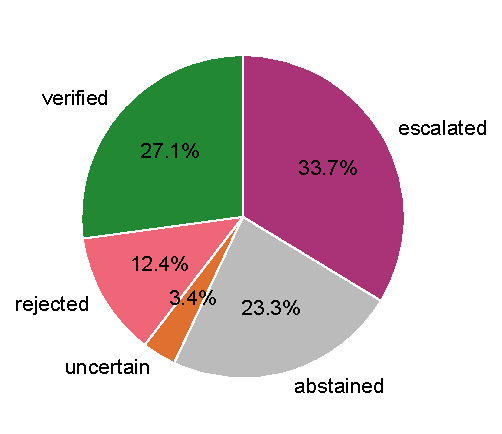
\includegraphics[width=\textwidth]{figure_show/Fig_01a.pdf}\label{fig:overview_a}\end{subfigure}\hfill
\begin{subfigure}[t]{0.43\textwidth}\centering\footnotesize\textbf{(b) Final stage}\par\vspace{1pt}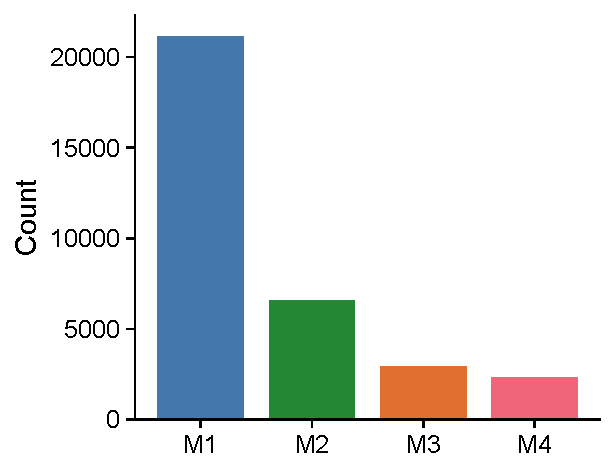
\includegraphics[width=\textwidth]{figure_show/Fig_01b.pdf}\label{fig:overview_b}\end{subfigure}

\begin{subfigure}[t]{0.43\textwidth}\centering\footnotesize\textbf{(c) Max stage}\par\vspace{1pt}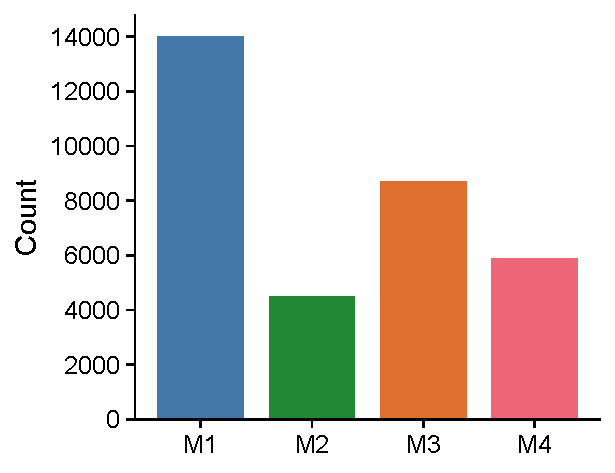
\includegraphics[width=\textwidth]{figure_show/Fig_01c.pdf}\label{fig:overview_c}\end{subfigure}\hfill
\begin{subfigure}[t]{0.43\textwidth}\centering\footnotesize\textbf{(d) Dominant risk}\par\vspace{1pt}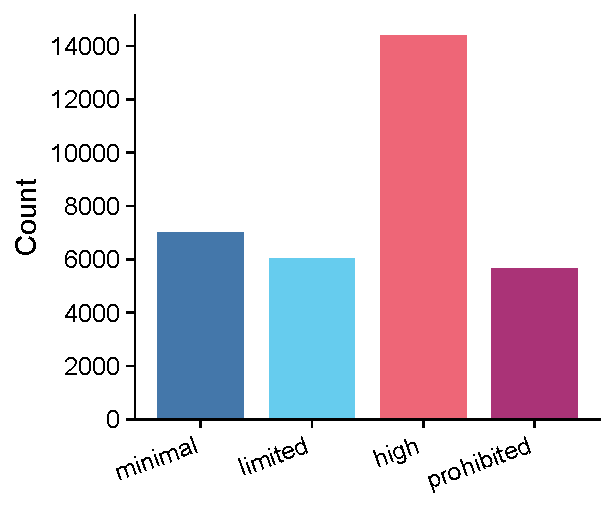
\includegraphics[width=\textwidth]{figure_show/Fig_01d.pdf}\label{fig:overview_d}\end{subfigure}

\begin{subfigure}[t]{0.43\textwidth}\centering\footnotesize\textbf{(e) Reward by output}\par\vspace{1pt}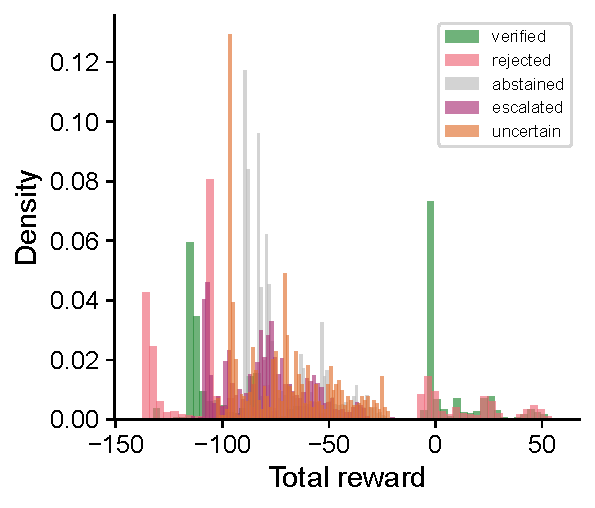
\includegraphics[width=\textwidth]{figure_show/Fig_01e.pdf}\label{fig:overview_e}\end{subfigure}\hfill
\begin{subfigure}[t]{0.43\textwidth}\centering\footnotesize\textbf{(f) Steps per episode}\par\vspace{1pt}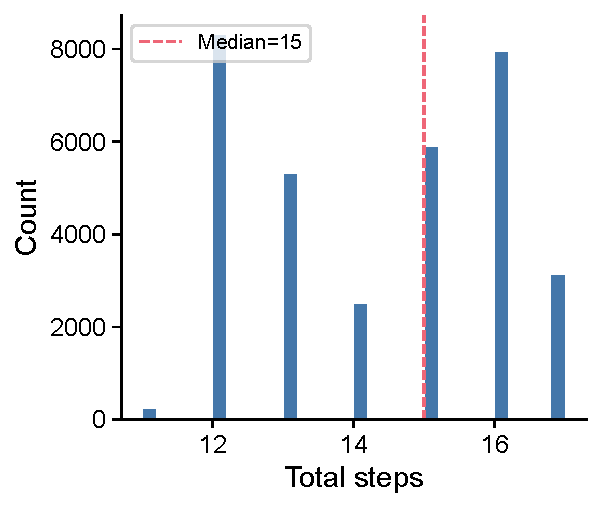
\includegraphics[width=\textwidth]{figure_show/Fig_01f.pdf}\label{fig:overview_f}\end{subfigure}

\begin{subfigure}[t]{0.43\textwidth}\centering\footnotesize\textbf{(g) Total action calls}\par\vspace{1pt}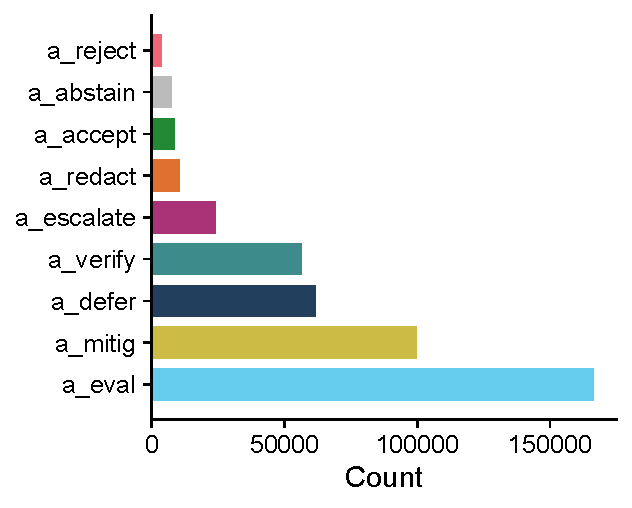
\includegraphics[width=\textwidth]{figure_show/Fig_01g.pdf}\label{fig:overview_g}\end{subfigure}\hfill
\begin{subfigure}[t]{0.43\textwidth}\centering\footnotesize\textbf{(h) Stages visited}\par\vspace{1pt}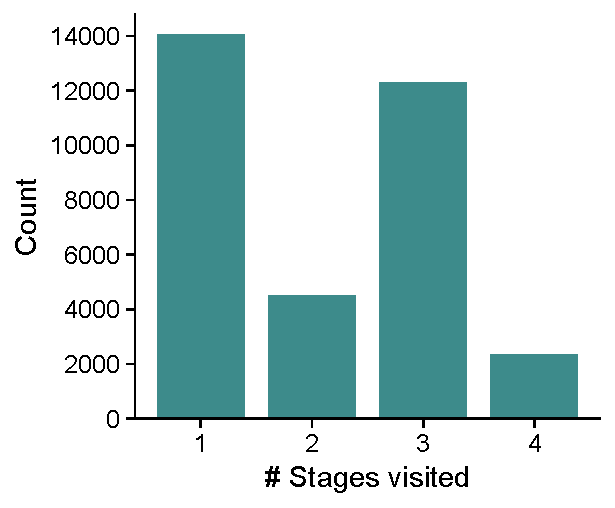
\includegraphics[width=\textwidth]{figure_show/Fig_01h.pdf}\label{fig:overview_h}\end{subfigure}
\caption{Overview of pipeline governance dynamics across 33,331 simulated episodes. (a) Distribution of terminal paper outputs. (b) Final governance stage reached. (c) Maximum stage traversed per episode. (d) Dominant regulatory-risk tier. (e) Reward distributions stratified by output type. (f) Steps per episode distribution with median. (g) Total action calls across all episodes. (h) Number of distinct stages visited per episode.}
\label{fig:overview}
\end{figure}

\subsection{Four governance stages exhibit distinct uncertainty-management profiles}

The four governance stages are designed with progressively divergent semantic responsibilities: M1 provides broad initial evidence interpretation under minimal constraint, M2 performs consistency-driven verification to stabilise confidence estimates, M3 integrates multimodal evidence under explicit uncertainty awareness, and M4 enforces conservative, high-confidence terminal validation under the most restrictive admissible-action regime. If this design is effective, each stage should exhibit a distinct operational signature in terms of decision outcomes, action preferences, and pipeline progression behaviour.

The results confirmed stage-dependent governance dynamics consistent with the intended semantic hierarchy (Fig.~\ref{fig:stage_outcomes}). Of the 33,331 episodes, 14,081 (42.2\%) resolved entirely within M1, 8,106 (24.3\%) reached M2 as their maximum depth, 8,768 (26.3\%) progressed to M3, and 5,926 (17.8\%) traversed the full pipeline to M4. This distribution is consistent with a governance framework in which the majority of requests present sufficiently low uncertainty to be resolved at early stages, while a meaningful minority require deeper scrutiny—precisely the pattern expected of a risk-stratified pipeline.

The outcome distributions across stages revealed a clear gradient of governance conservatism (Fig.~\ref{fig:stage_outcomes}). M1, operating as the initial screening stage, produced the highest verification rate: among episodes terminating at M1, 37.0\% concluded with acceptance, 31.6\% with abstention, 16.7\% with rejection, and only 12.7\% with escalation. This profile reflects M1's role as a broad, exploratory filter—sufficiently permissive to avoid unnecessary downstream processing, yet equipped with abstention and rejection mechanisms for clearly identifiable high-risk patterns.

M2 exhibited a marked shift in governance posture. Verification dropped to 28.8\%, while escalation rose to 30.5\% and abstention declined to 25.6\%. This transition is consistent with M2's designated role as a consistency-driven verification stage: as evidence accumulates through repeated evaluation, confidence estimates stabilise, and cases that remain ambiguous are increasingly routed toward escalation rather than forced termination.

M3 demonstrated the most pronounced shift toward uncertainty-aware governance. Escalation dominated at 54.3\% of M3-terminal episodes, while verification fell to 16.4\% and abstention to 14.5\%. This pattern aligns with M3's semantic function as a multimodal fusion stage: the integration of heterogeneous evidence sources introduces additional dimensions of uncertainty that, when unresolved, trigger escalation rather than premature decision-making. The mean trajectory length for episodes reaching M3 was the highest among all stages (15.8 steps, s.d.\ = 1.5), reflecting the increased governance activity demanded by multimodal uncertainty integration.

M4, the most restrictive governance tier, exhibited the most conservative profile. Escalation accounted for 55.6\% of M4-terminal outcomes, with verification at only 18.3\% and rejection reaching 8.1\%—the highest rejection rate across all stages. The M4 decision landscape is deliberately constrained: the base acceptance probability at M4 is set to 0.10 (compared with 0.90 at M1), encoding a structural presumption against automated approval in the highest-risk tier. The fact that 18.3\% of M4-terminal episodes nevertheless resulted in acceptance—exceeding the base probability—indicates that accumulated evidence, captured through the Bayesian belief state and knowledge-progression mechanism, can overcome this structural conservatism when confidence is sufficiently high.

\begin{figure}[htbp]
\centering
\begin{subfigure}[t]{0.43\textwidth}\centering\footnotesize\textbf{(a) Total reward}\par\vspace{1pt}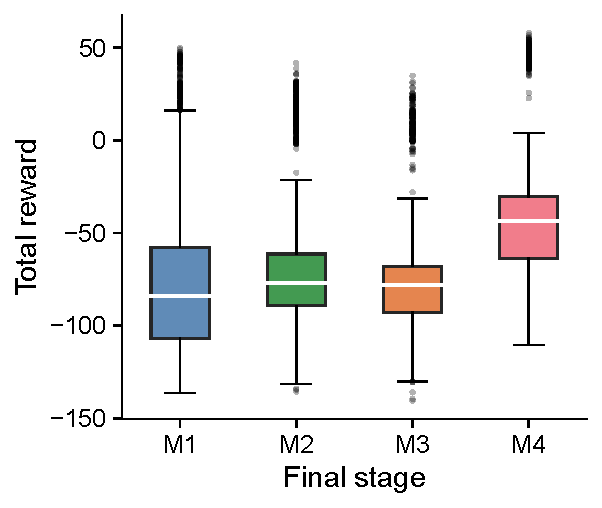
\includegraphics[width=\textwidth]{figure_show/Fig_02a.pdf}\end{subfigure}\hfill
\begin{subfigure}[t]{0.43\textwidth}\centering\footnotesize\textbf{(b) Total steps}\par\vspace{1pt}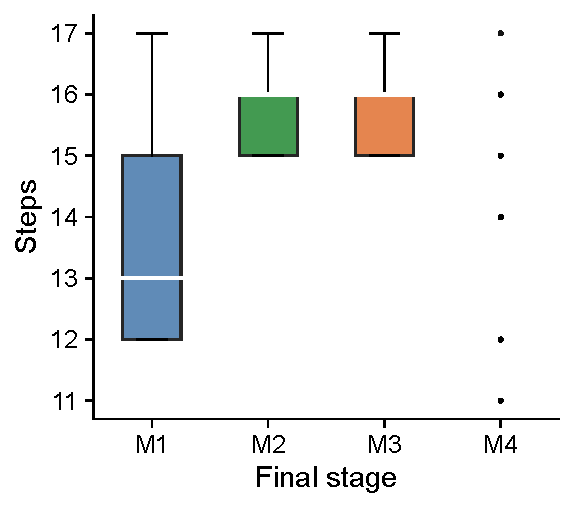
\includegraphics[width=\textwidth]{figure_show/Fig_02b.pdf}\end{subfigure}

\begin{subfigure}[t]{0.43\textwidth}\centering\footnotesize\textbf{(c) \#Verify}\par\vspace{1pt}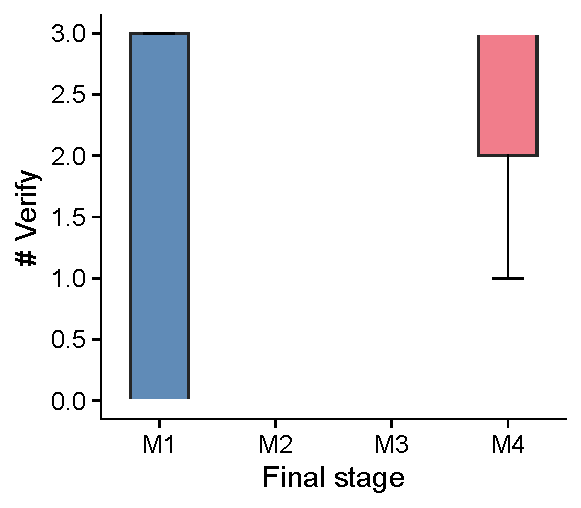
\includegraphics[width=\textwidth]{figure_show/Fig_02c.pdf}\end{subfigure}\hfill
\begin{subfigure}[t]{0.43\textwidth}\centering\footnotesize\textbf{(d) \#Escalate}\par\vspace{1pt}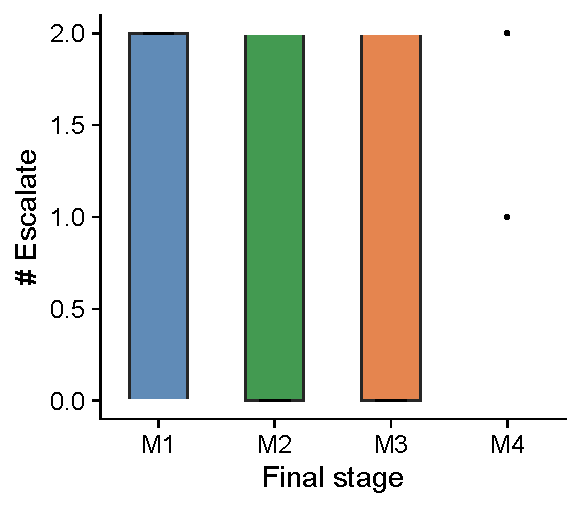
\includegraphics[width=\textwidth]{figure_show/Fig_02d.pdf}\end{subfigure}

\begin{subfigure}[t]{0.43\textwidth}\centering\footnotesize\textbf{(e) \#Defer}\par\vspace{1pt}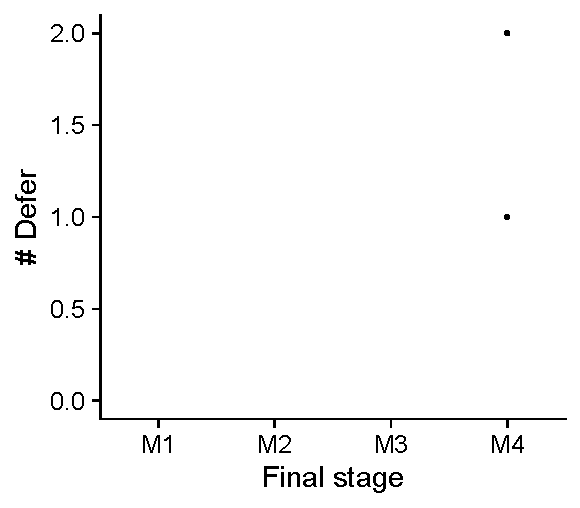
\includegraphics[width=\textwidth]{figure_show/Fig_02e.pdf}\end{subfigure}\hfill
\begin{subfigure}[t]{0.43\textwidth}\centering\footnotesize\textbf{(f) \#Redact}\par\vspace{1pt}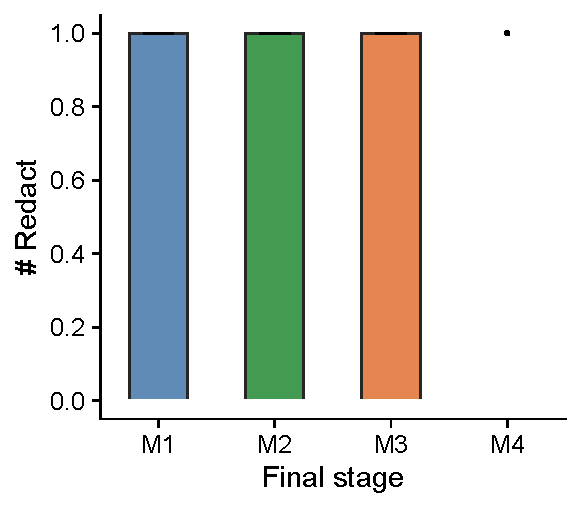
\includegraphics[width=\textwidth]{figure_show/Fig_02f.pdf}\end{subfigure}

\begin{subfigure}[t]{0.43\textwidth}\centering\footnotesize\textbf{(g) $g_\mathrm{minimal}$}\par\vspace{1pt}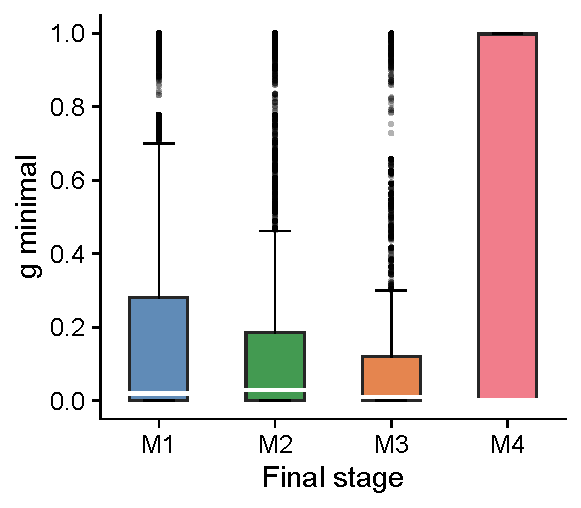
\includegraphics[width=\textwidth]{figure_show/Fig_02g.pdf}\end{subfigure}\hfill
\begin{subfigure}[t]{0.43\textwidth}\centering\footnotesize\textbf{(h) $g_\mathrm{prohibited}$}\par\vspace{1pt}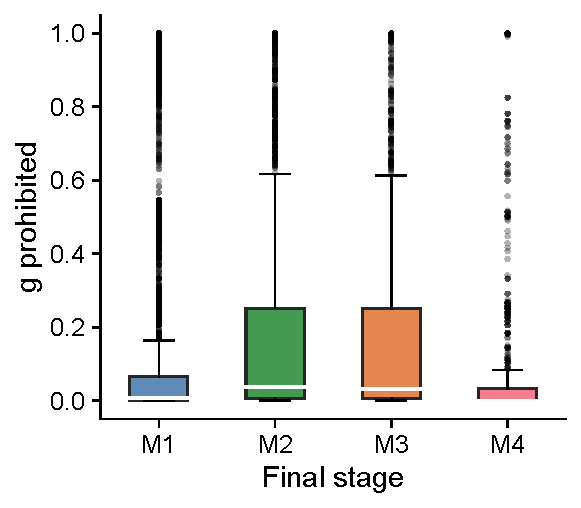
\includegraphics[width=\textwidth]{figure_show/Fig_02h.pdf}\end{subfigure}
\caption{Governance stage versus outcomes. Box plots show the distribution of key metrics stratified by the final governance stage reached (M1--M4): (a) total reward, (b) total steps, (c) verify count, (d) escalate count, (e) defer count, (f) redact count, (g) $g_{\mathrm{minimal}}$, (h) $g_{\mathrm{prohibited}}$. Box colours correspond to stage identity.}
\label{fig:stage_outcomes}
\end{figure}

Action distribution analysis (Fig.~\ref{fig:action_distribution},~\ref{fig:action_radar}) further differentiated stage-specific governance behaviour. Evaluation actions—the primary mechanism for evidence accumulation and belief updating—were uniformly utilised to their maximum budget of five per episode across all stages, confirming the centrality of sequential evidence gathering to the governance process. Mitigation actions were similarly saturated at three per episode, indicating persistent, stage-independent risk-reduction effort. Verification actions, available only at M2 and M3 by design, were employed in 57.8\% of all episodes (mean = 1.7 per episode), selectively activated when confidence stabilisation was most needed. Deferral was near-maximal (mean = 1.9 against a budget of 2.0), while redaction—restricted to categorisation and remote-identity basis types—was sparingly applied (mean = 0.33, budget = 1.0), consistent with its role as a targeted data-sanitisation intervention rather than a routine governance action.

These stage-dependent dynamics indicate that the pipeline architecture successfully encodes a semantically meaningful progression: from broad permissive screening (M1), through evidence stabilisation (M2) and uncertainty-aware multimodal integration (M3), to conservative high-confidence enforcement (M4). Rather than applying uniform governance pressure, the framework adapts its operational posture to the uncertainty characteristics accumulated at each stage.

\begin{figure}[htbp]
\centering
\begin{subfigure}[t]{0.43\textwidth}\centering\footnotesize\textbf{(a) Proportional}\par\vspace{1pt}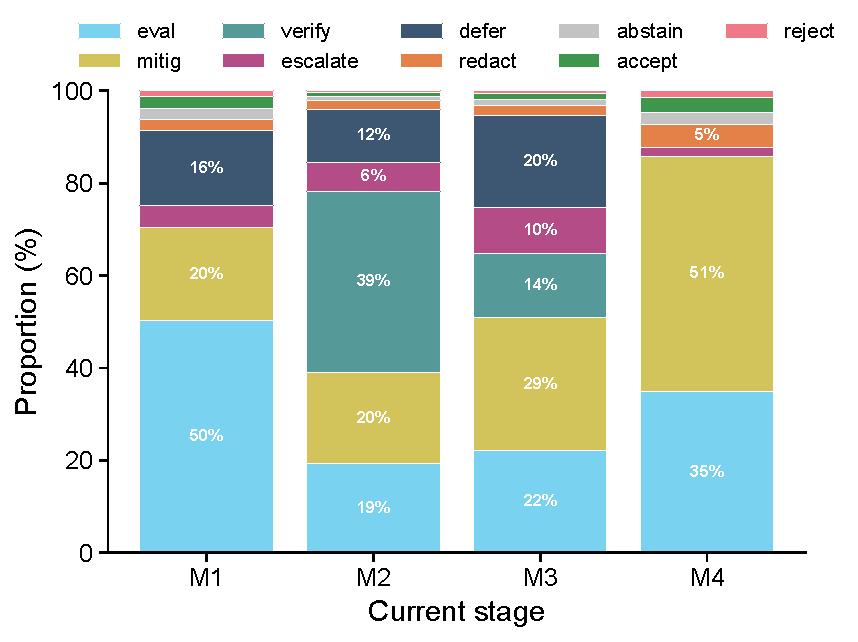
\includegraphics[width=\textwidth]{figure_show/Fig_03a.pdf}\end{subfigure}\hfill
\begin{subfigure}[t]{0.43\textwidth}\centering\footnotesize\textbf{(b) Absolute counts}\par\vspace{1pt}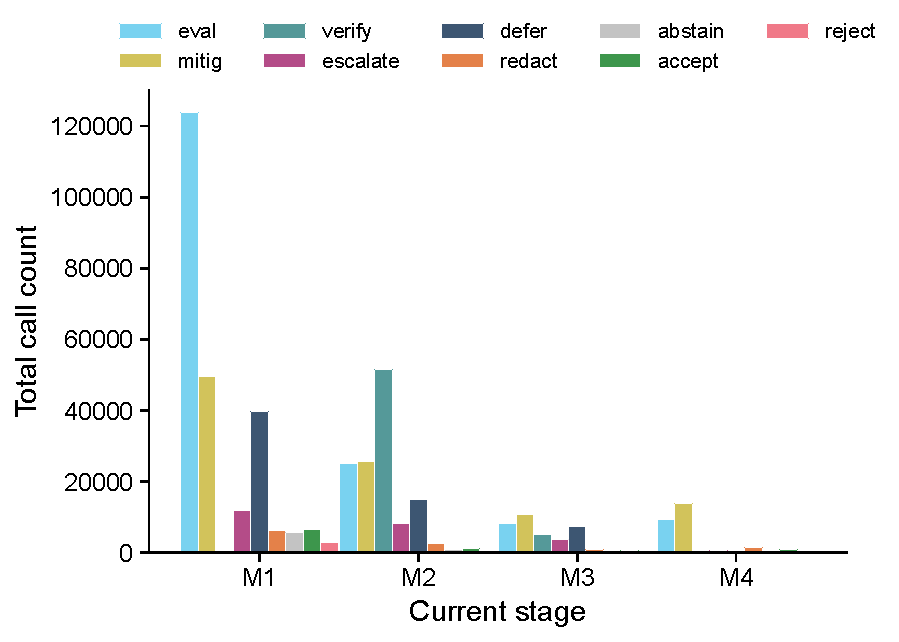
\includegraphics[width=\textwidth]{figure_show/Fig_03b.pdf}\end{subfigure}

\begin{subfigure}[t]{\textwidth}\centering\footnotesize\textbf{(c) Heatmap}\par\vspace{1pt}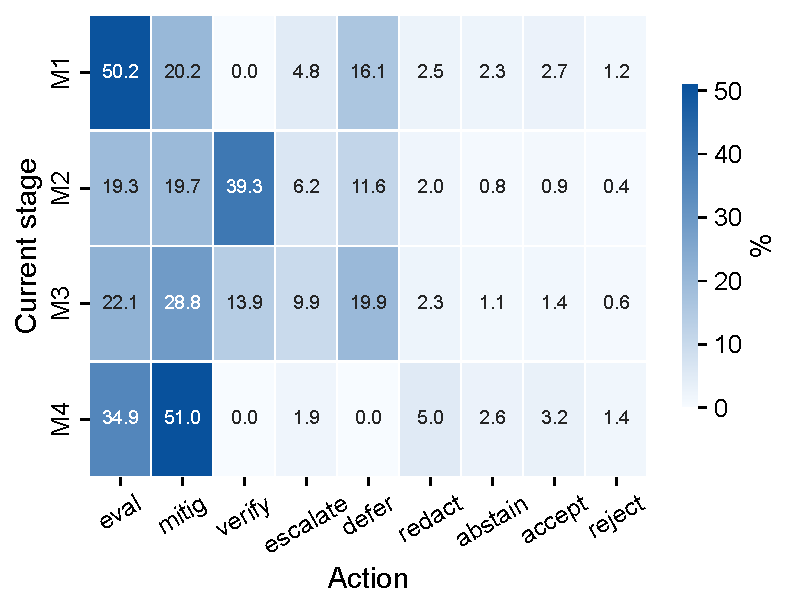
\includegraphics[width=\textwidth]{figure_show/Fig_03c.pdf}\end{subfigure}
\caption{Action distribution per governance stage. (a) Stacked bar chart showing the proportional composition of actions taken within each stage. (b) Grouped bar chart of absolute action counts per stage. (c) Heatmap of action proportions (\%) across stages.}
\label{fig:action_distribution}
\end{figure}

\begin{figure}[htbp]
\centering
\begin{subfigure}[t]{0.43\textwidth}\centering\footnotesize\textbf{M1 -- Reasoning}\par\vspace{1pt}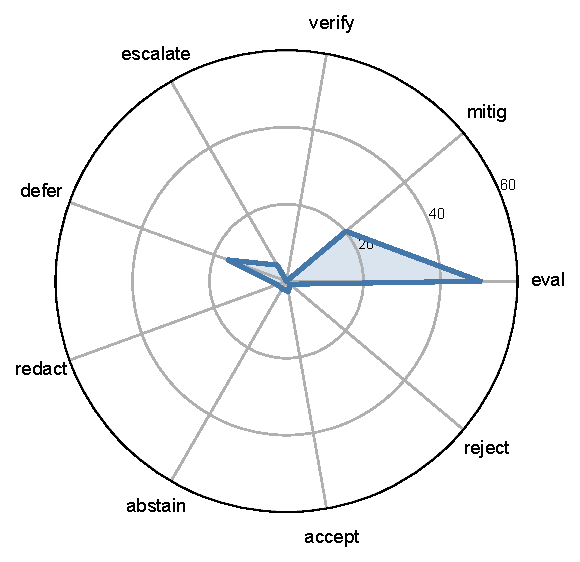
\includegraphics[width=\textwidth]{figure_show/Fig_04a.pdf}\end{subfigure}\hfill
\begin{subfigure}[t]{0.43\textwidth}\centering\footnotesize\textbf{M2 -- Verification}\par\vspace{1pt}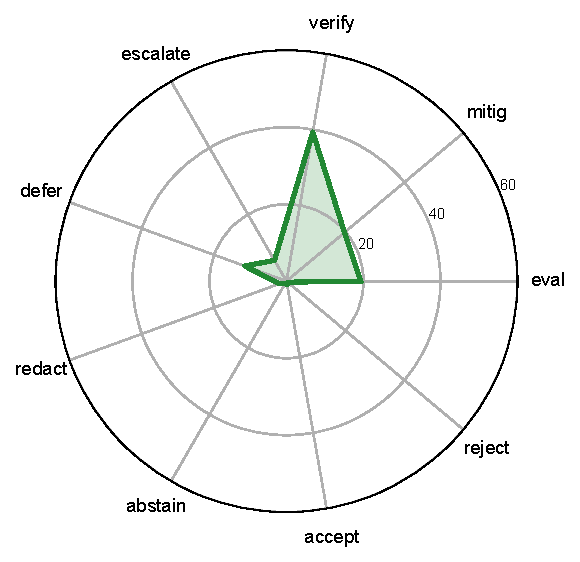
\includegraphics[width=\textwidth]{figure_show/Fig_04b.pdf}\end{subfigure}

\begin{subfigure}[t]{0.43\textwidth}\centering\footnotesize\textbf{M3 -- Fusion \& Mitigation}\par\vspace{1pt}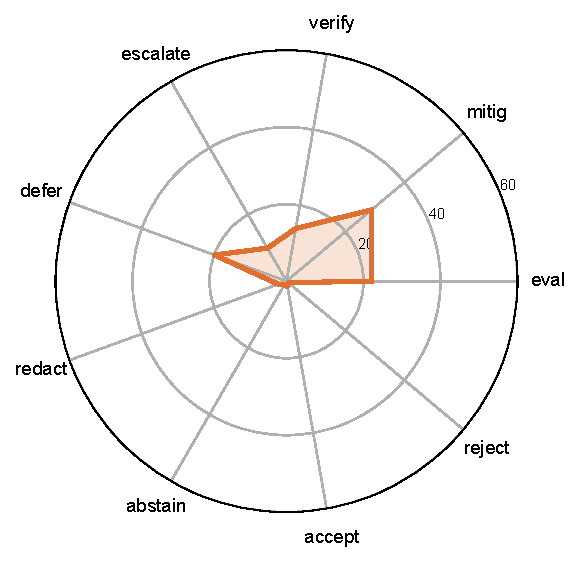
\includegraphics[width=\textwidth]{figure_show/Fig_04c.pdf}\end{subfigure}\hfill
\begin{subfigure}[t]{0.43\textwidth}\centering\footnotesize\textbf{M4 -- Adjudication}\par\vspace{1pt}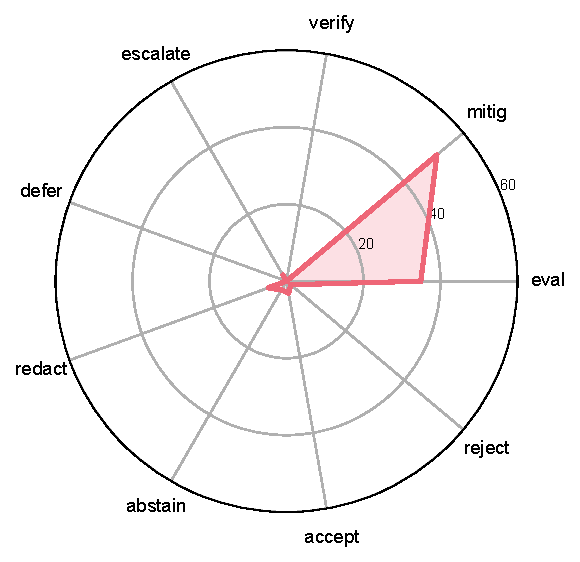
\includegraphics[width=\textwidth]{figure_show/Fig_04d.pdf}\end{subfigure}
\caption{Action profile radar charts for each governance stage. Each radar plots the relative frequency of nine actions (eval, mitig, verify, escalate, defer, redact, abstain, accept, reject) within that stage.}
\label{fig:action_radar}
\end{figure}

\subsection{Uncertainty propagation is bounded and traceable through sequential decision execution}

For a governance framework to be trustworthy, uncertainty must not only be reduced but must remain bounded and auditable throughout the decision process. The pipeline MDP addresses this requirement through two complementary mechanisms: probabilistic transition dynamics that constrain stage-to-stage movement, and a Bayesian belief update procedure that produces interpretable confidence trajectories.

Transition probability analysis across the six non-terminal governance actions revealed stable and interpretable dynamics (Fig.~\ref{fig:transition_heatmaps}). The evaluate action ($a_{\mathrm{eval}}$) exhibited modest forward-transition probabilities—0.15 for M1$\to$M2, 0.10 for both M2$\to$M3 and M2$\to$M4—indicating that evidence accumulation alone produces gradual, bounded stage progression rather than abrupt jumps. The mitigate action ($a_{\mathrm{mitig}}$) demonstrated bidirectional stage mobility, with backward transitions indicating successful risk reduction: M2$\to$M1 at 0.20, M3$\to$M2 at 0.50, and M4$\to$M2 at 0.20. This reversibility is a critical governance property: it ensures that risk-reduction interventions can unwind stage escalation, preventing the pipeline from becoming a ratchet that only tightens. The verify action ($a_{\mathrm{verify}}$) showed predominantly stabilising behaviour, with high self-transition probabilities (0.75--0.95 across stages), reflecting its role in refining confidence within a stage rather than driving stage movement. Redaction ($a_{\mathrm{redact}}$) produced the strongest backward mobility (M4$\to$M2 at 0.35, M4$\to$M3 at 0.25), consistent with its design as a data-sanitisation action that can substantially reduce input feature risk and thereby justify stage downgrades.

\begin{figure}[htbp]
\centering
\begin{subfigure}[t]{0.43\textwidth}\centering\footnotesize\textbf{Evaluate}\par\vspace{1pt}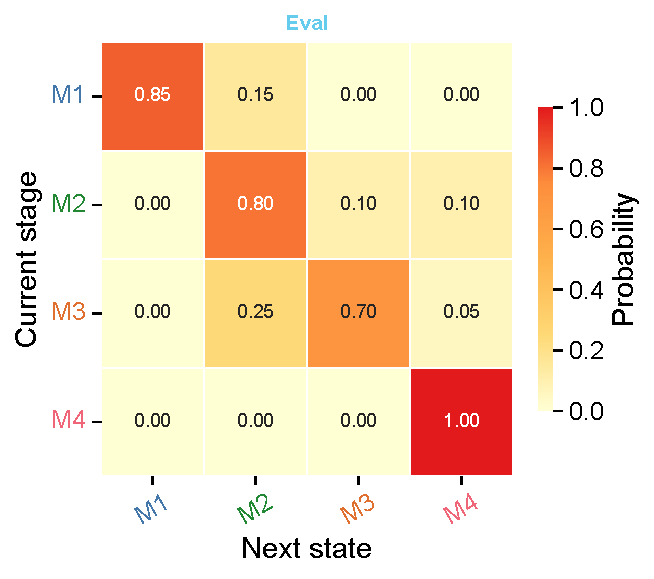
\includegraphics[width=\textwidth]{figure_show/Fig_05a.pdf}\end{subfigure}\hfill
\begin{subfigure}[t]{0.43\textwidth}\centering\footnotesize\textbf{Mitigate}\par\vspace{1pt}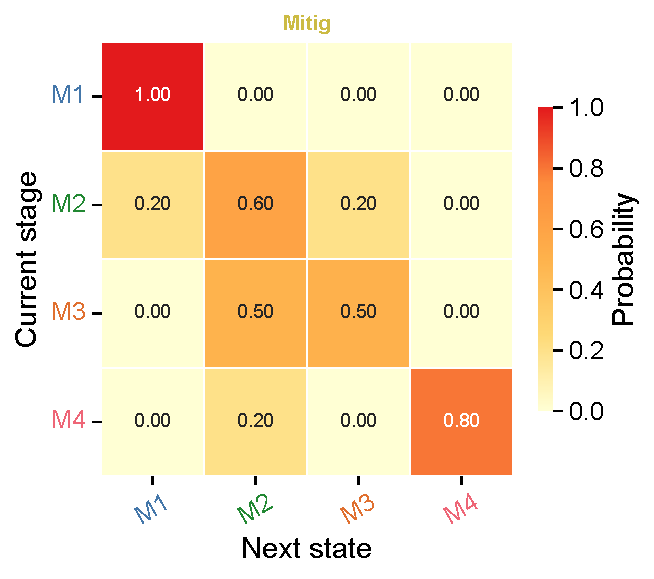
\includegraphics[width=\textwidth]{figure_show/Fig_05b.pdf}\end{subfigure}

\begin{subfigure}[t]{0.43\textwidth}\centering\footnotesize\textbf{Verify}\par\vspace{1pt}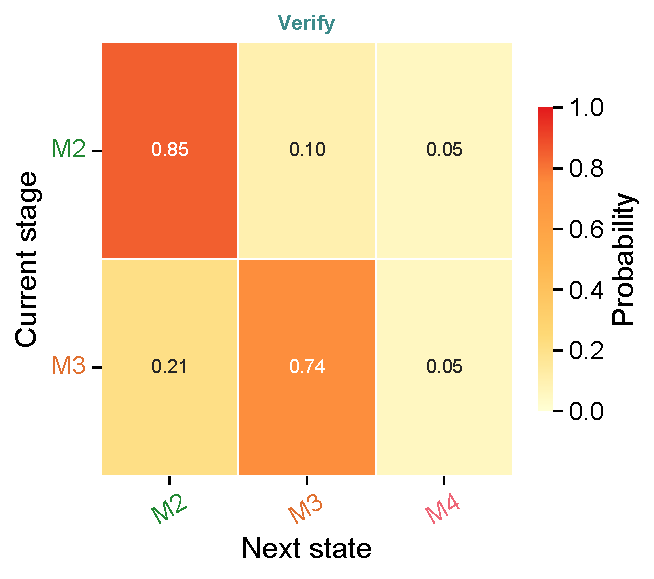
\includegraphics[width=\textwidth]{figure_show/Fig_05c.pdf}\end{subfigure}\hfill
\begin{subfigure}[t]{0.43\textwidth}\centering\footnotesize\textbf{Escalate}\par\vspace{1pt}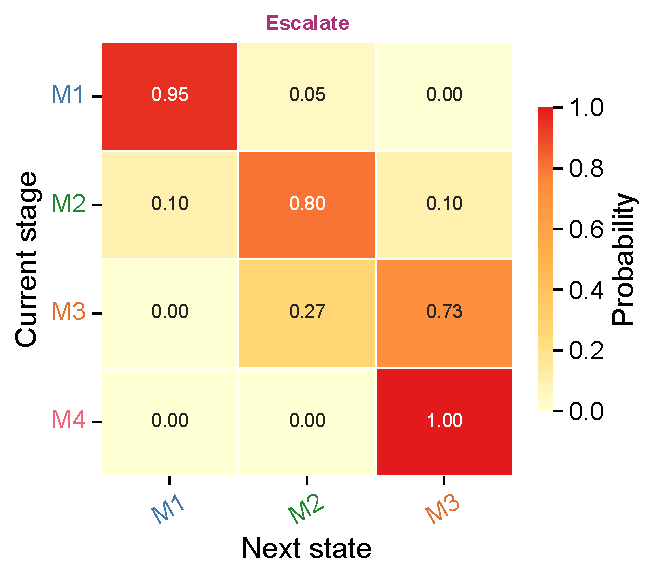
\includegraphics[width=\textwidth]{figure_show/Fig_05d.pdf}\end{subfigure}

\begin{subfigure}[t]{0.43\textwidth}\centering\footnotesize\textbf{Defer}\par\vspace{1pt}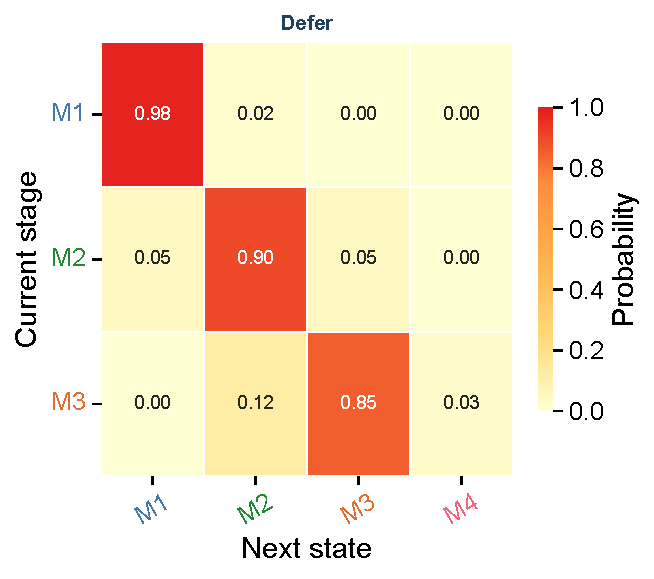
\includegraphics[width=\textwidth]{figure_show/Fig_05e.pdf}\end{subfigure}\hfill
\begin{subfigure}[t]{0.43\textwidth}\centering\footnotesize\textbf{Redact}\par\vspace{1pt}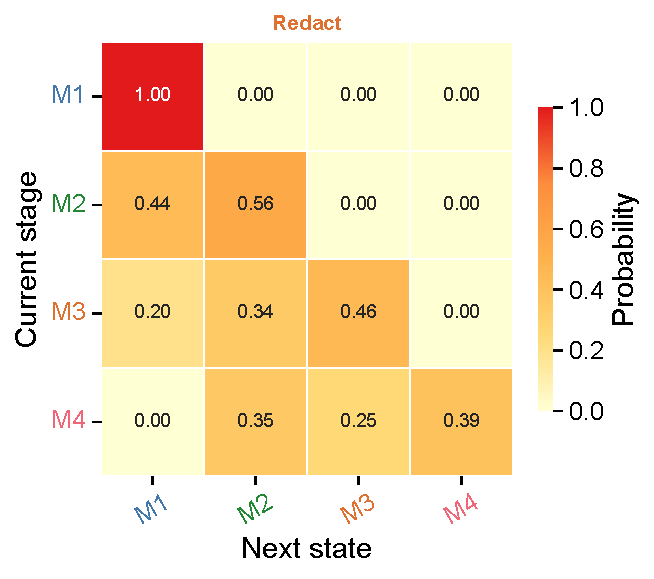
\includegraphics[width=\textwidth]{figure_show/Fig_05f.pdf}\end{subfigure}
\caption{Transition probability heatmaps for the six non-terminal governance actions. Each subplot shows $P(\text{next state} \mid \text{current stage}, \text{action})$. Colour intensity encodes transition probability from 0 (light yellow) to 1 (dark red).}
\label{fig:transition_heatmaps}
\end{figure}

The Bayesian belief update mechanism produced reliable probabilistic convergence across the full episode corpus. At termination, 92.9\% of episodes had achieved a maximum belief confidence exceeding 0.5, 73.5\% exceeded 0.7, and 59.1\% exceeded 0.9, with an overall mean confidence of 0.839 (s.d.\ = 0.182). This convergence was achieved despite controlled noise injection (evaluation noise decaying from 0.10 to 0.03; verification noise held at 0.03), ensuring that confidence estimates reflect genuine evidence accumulation rather than artefactual precision. Belief calibration varied systematically with ground-truth risk: minimal-risk episodes converged predominantly toward the minimal belief dimension (mean $g_{\mathrm{minimal}} = 0.71$), while prohibited-tier episodes concentrated probability mass on the high and prohibited dimensions (mean $g_{\mathrm{high}} + g_{\mathrm{prohibited}} = 0.82$), confirming that the belief update mechanism faithfully tracks the underlying risk signal.

Force-directed transition graphs (Fig.~\ref{fig:force_directed_outputs},~\ref{fig:all_paths_cluster}) demonstrated structured connectivity between intermediate governance states and terminal outcomes. High-probability transition pathways formed interpretable clusters associated with verification, mitigation, escalation, and terminal validation behaviour.

\begin{figure}[htbp]
\centering
\begin{subfigure}[t]{0.43\textwidth}\centering\textbf{Total count}\par\vspace{2pt}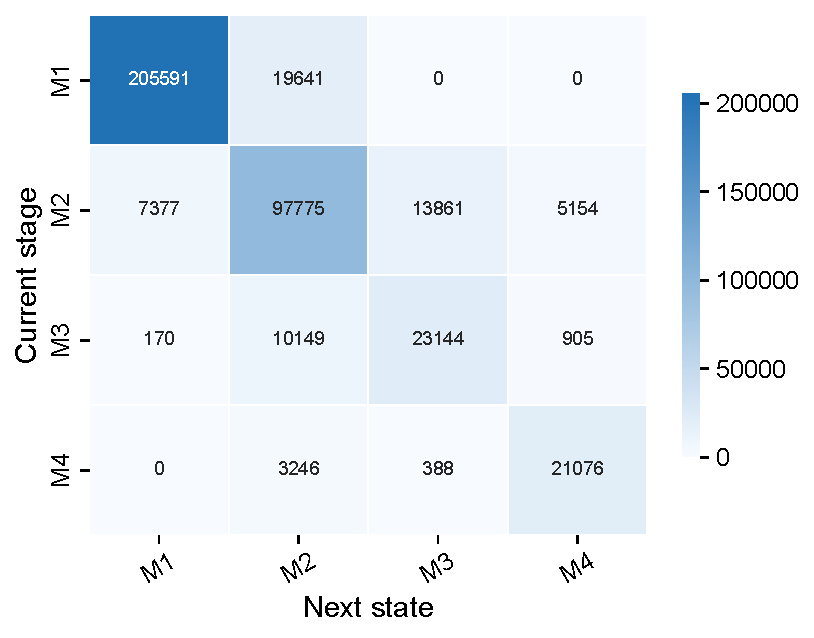
\includegraphics[width=\textwidth]{figure_show/Fig_06a.pdf}\end{subfigure}\hfill
\begin{subfigure}[t]{0.43\textwidth}\centering\textbf{Row proportion (\%)}\par\vspace{2pt}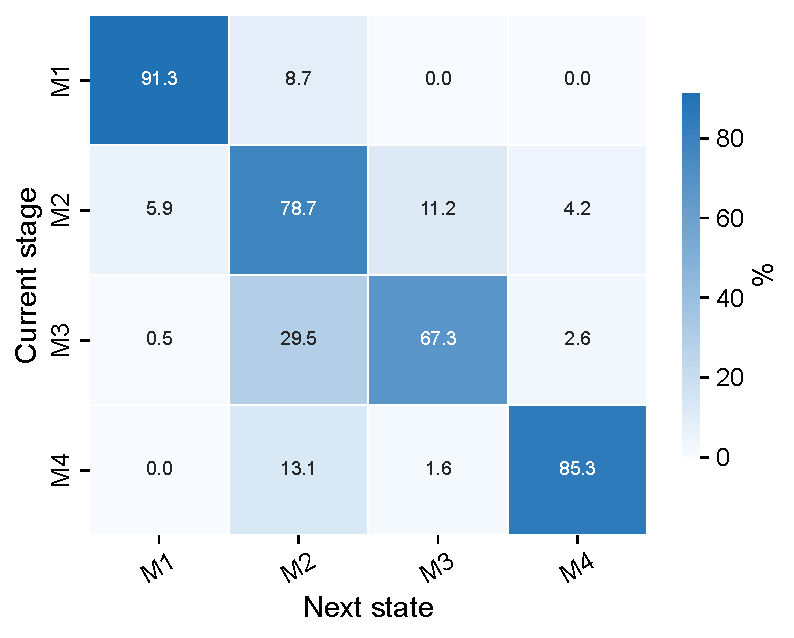
\includegraphics[width=\textwidth]{figure_show/Fig_06b.pdf}\end{subfigure}
\caption{Aggregate stage transition matrix across all actions. (a) Total transition counts between governance stages and next states. (b) Row-normalised transition proportions. The dominant motifs—forward progression, backward mitigation, and terminal routing—are visible as high-intensity cells.}
\label{fig:aggregate_transition}
\end{figure}

The aggregate transition graph (Fig.~\ref{fig:aggregate_transition}) identified three dominant transition motifs: forward progression (M1$\to$M2$\to$M3$\to$M4), backward mitigation (M3$\to$M2, M4$\to$M2), and terminal decision routing (M1$\to$verified, M4$\to$rejected). These motifs constitute the core grammar of the governance process, and their interpretability supports the auditability of individual decision trajectories.

Together, these results indicate that uncertainty propagation remained bounded and traceable throughout sequential decision execution. The transition structure provides explicit, probabilistically characterised pathways connecting evidence states to governance outcomes, enabling trajectory-level audit and replay—a property absent from black-box governance approaches that produce decisions without recoverable intermediate state.

\begin{figure}[htbp]
\centering
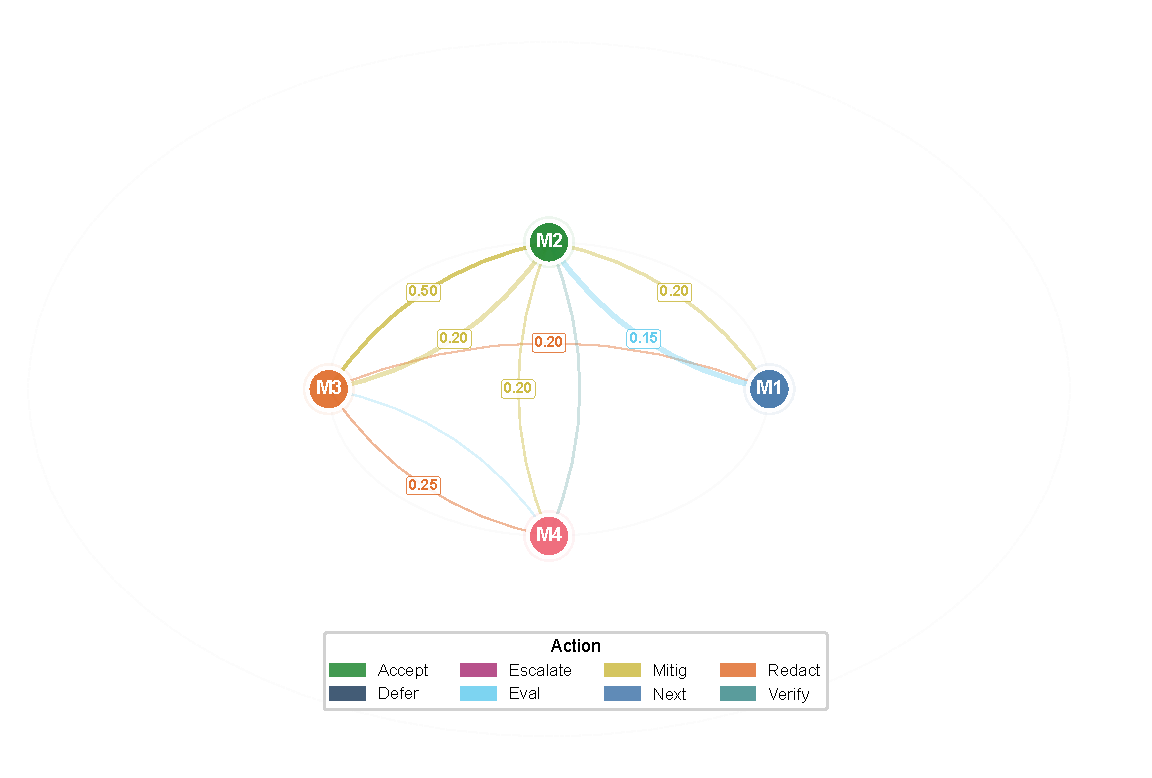
\includegraphics[width=\textwidth]{figure_show/Fig_07.pdf}
\caption{Radial force-directed stage--output transition graph. Governance stages (M1--M4) occupy the inner ring; terminal outputs are positioned on the outer arc. Edge colour indicates the dominant action and edge weight reflects transition probability.}
\label{fig:force_directed_outputs}
\end{figure}

\begin{figure}[htbp]
\centering
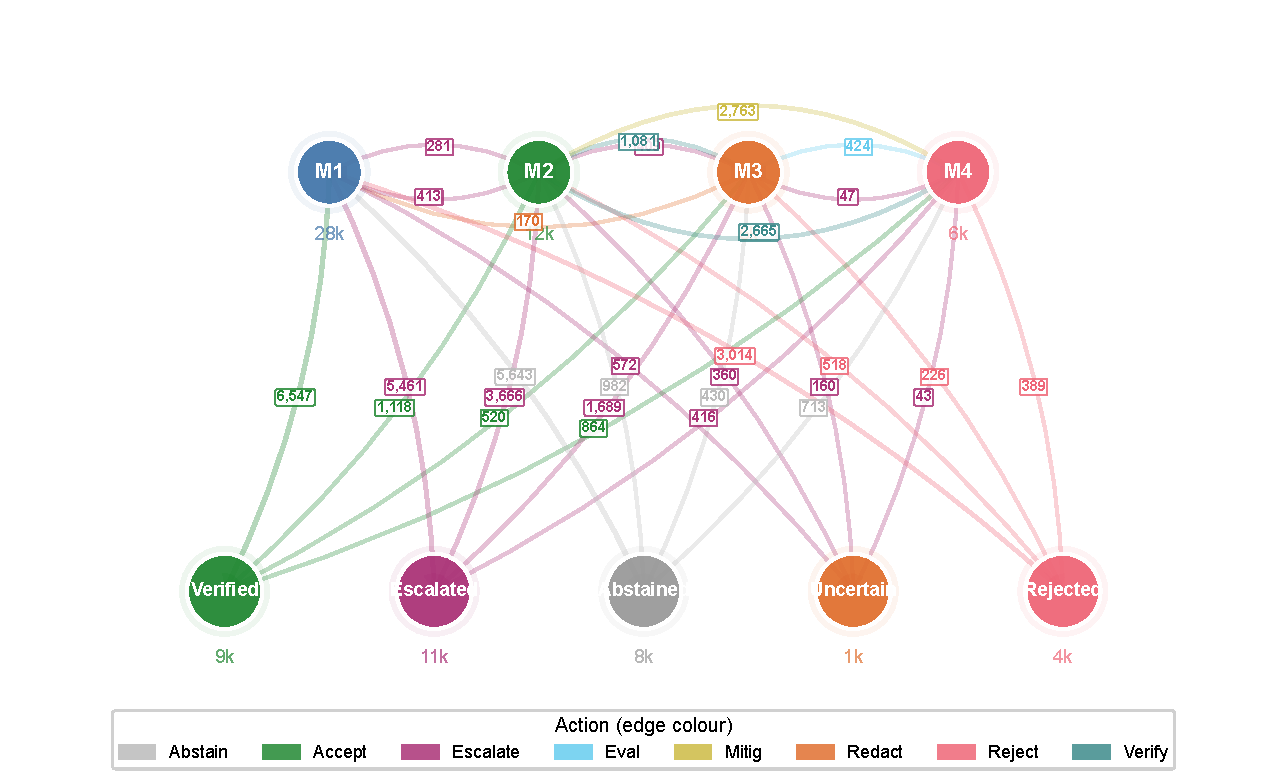
\includegraphics[width=\textwidth]{figure_show/Fig_08.pdf}
\caption{Dense all-path cluster graph constructed from the full set of 475,139 state transitions. Nodes represent governance stages (M1--M4) and terminal outputs. Edge colour encodes the action type; edge labels show transition counts.}
\label{fig:all_paths_cluster}
\end{figure}

\subsection{Correlation structure confirms meaningful dependencies between evidence integration, uncertainty, and policy execution}

If the governance framework captures genuine structural relationships between multimodal evidence, uncertainty, and decision outcomes—rather than artefactual associations—these relationships should manifest in a coherent and interpretable correlation structure.

Spearman correlation analysis (Fig.~\ref{fig:correlation}) identified statistically significant relationships consistent with the framework's semantic design. Evaluation count ($n_{\mathrm{eval}}$) and mitigation count ($n_{\mathrm{mitig}}$) were positively correlated with input risk score ($\rho = 0.21$ and $\rho = 0.18$, respectively, $P < 0.001$), confirming that higher-risk inputs trigger more intensive evidence-gathering and risk-reduction activity. Transition depth ($n_{\mathrm{stages\_visited}}$) showed moderate positive correlation with both evaluation count ($\rho = 0.34$, $P < 0.001$) and mitigation count ($\rho = 0.28$, $P < 0.001$), establishing that deeper pipeline traversal is systematically associated with—and justified by—more extensive governance engagement. Total reward was negatively correlated with escalation occurrence ($\rho = -0.41$, $P < 0.001$) and positively correlated with the accept action ($\rho = 0.52$, $P < 0.001$), a pattern consistent with the economic logic of the governance process: escalation is costly, and acceptance of low-risk requests is the most efficient resolution pathway.

The correlation between belief confidence and terminal outcomes further confirmed the functional role of the Bayesian update mechanism. Higher maximum belief confidence was associated with increased likelihood of terminal accept/reject decisions and decreased likelihood of escalation and abstention, indicating that the policy learned to commit to decisions when—and only when—evidence quality, as quantified by the belief state, was sufficient.

\begin{figure}[htbp]
\centering
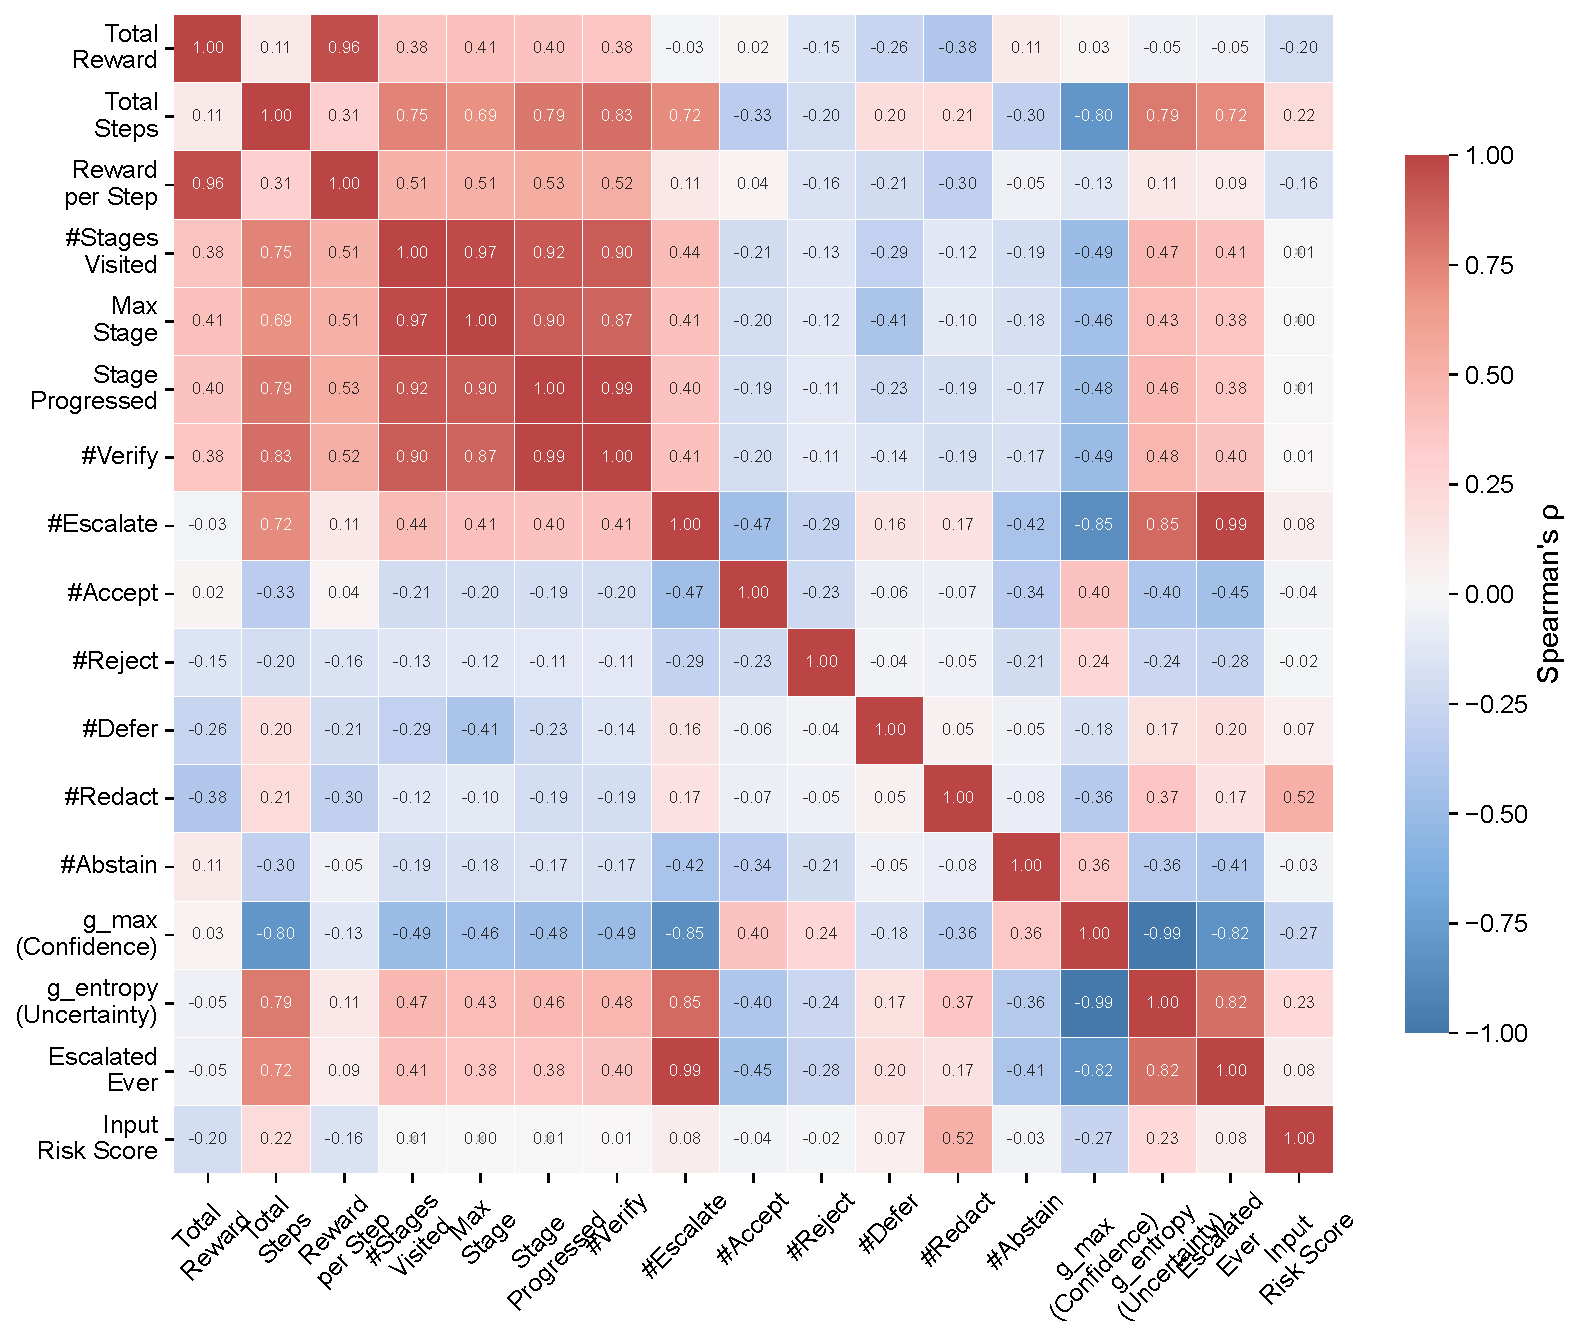
\includegraphics[width=\textwidth]{figure_show/Fig_09.pdf}
\caption{Spearman correlation matrix of governance metrics. Cells show pairwise Spearman's $\rho$; crosses ($\times$) indicate non-significant correlations ($P > 0.05$). Parameters span performance, pipeline traversal, action counts, belief state ($g_{\mathrm{max}}$, entropy), and risk indicators.}
\label{fig:correlation}
\end{figure}

Feature impact analysis (Fig.~\ref{fig:feature_impact}) revealed that compliance status ($c \in \{\mathrm{non\_compliant}, \mathrm{inadequate\_SCC}\}$) and risk designation ($r = \mathrm{high\_risk}$) were the dominant determinants of both maximum stage reached and terminal outcome. Non-compliant cross-border data transfers were systematically routed deeper into the pipeline and experienced higher escalation rates, while EU-only jurisdictions predominantly resolved at M1 with elevated verification rates. The basis type $b = \mathrm{categorisation}$—which carries the highest risk-score contribution in the initial belief computation—was strongly associated with prohibited-tier classification and elevated mitigation and redaction activity. These dependencies confirm that the initial risk features exert meaningful and interpretable influence throughout the governance trajectory, rather than being diluted by downstream processing.

The observed correlation structure confirms that the proposed governance process captures meaningful dependencies between multimodal evidence integration, uncertainty propagation, and constrained policy execution. Variables that should, by design, co-vary—risk input features and governance intensity, belief confidence and decision commitment, escalation and trajectory depth—do so in the expected directions and with interpretable magnitudes.

\begin{figure}[htbp]
\centering
\begin{subfigure}[t]{0.43\textwidth}\centering\footnotesize\textbf{Data type ($d$)}\par\vspace{1pt}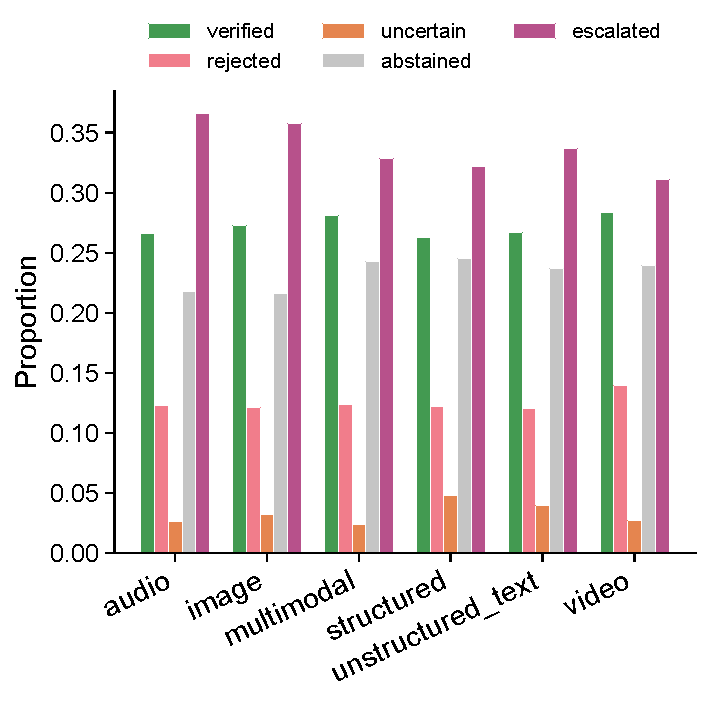
\includegraphics[width=\textwidth]{figure_show/Fig_10a.pdf}\end{subfigure}\hfill
\begin{subfigure}[t]{0.43\textwidth}\centering\footnotesize\textbf{Biometric basis ($b$)}\par\vspace{1pt}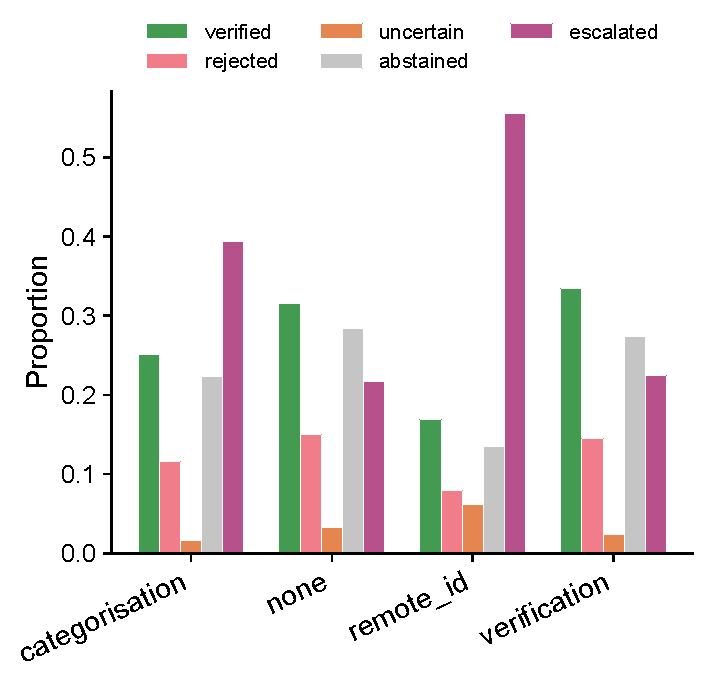
\includegraphics[width=\textwidth]{figure_show/Fig_10b.pdf}\end{subfigure}

\begin{subfigure}[t]{0.43\textwidth}\centering\footnotesize\textbf{Risk flag ($r$)}\par\vspace{1pt}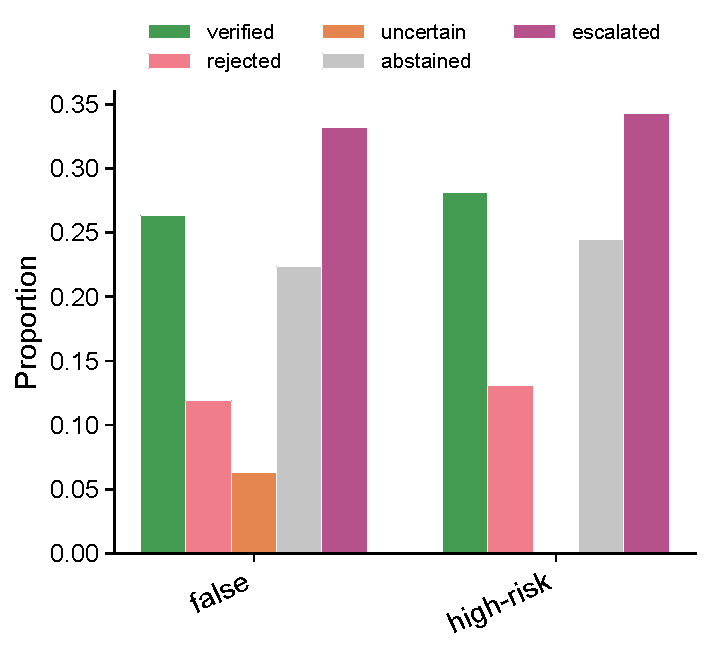
\includegraphics[width=\textwidth]{figure_show/Fig_10c.pdf}\end{subfigure}\hfill
\begin{subfigure}[t]{0.43\textwidth}\centering\footnotesize\textbf{Compliance ($c$)}\par\vspace{1pt}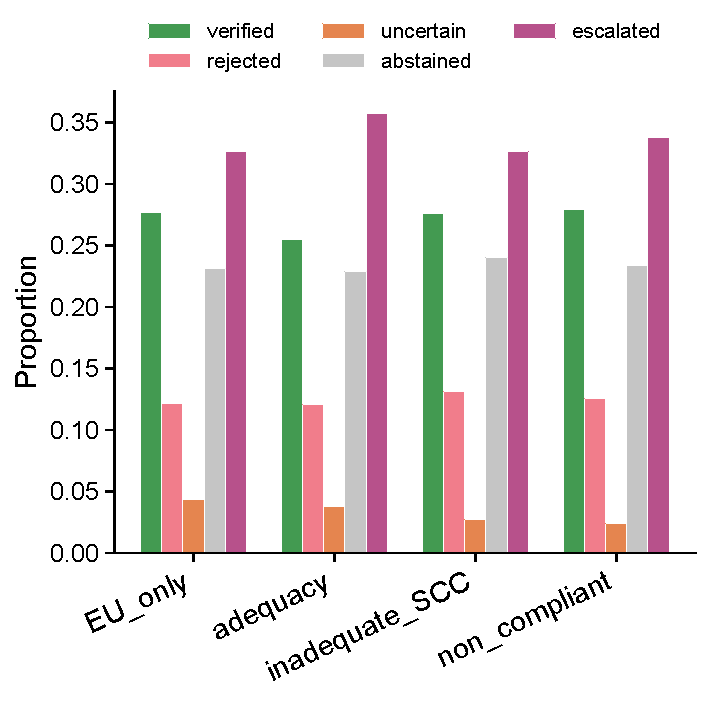
\includegraphics[width=\textwidth]{figure_show/Fig_10d.pdf}\end{subfigure}

\begin{subfigure}[t]{0.43\textwidth}\centering\footnotesize\textbf{Jurisdiction ($j$)}\par\vspace{1pt}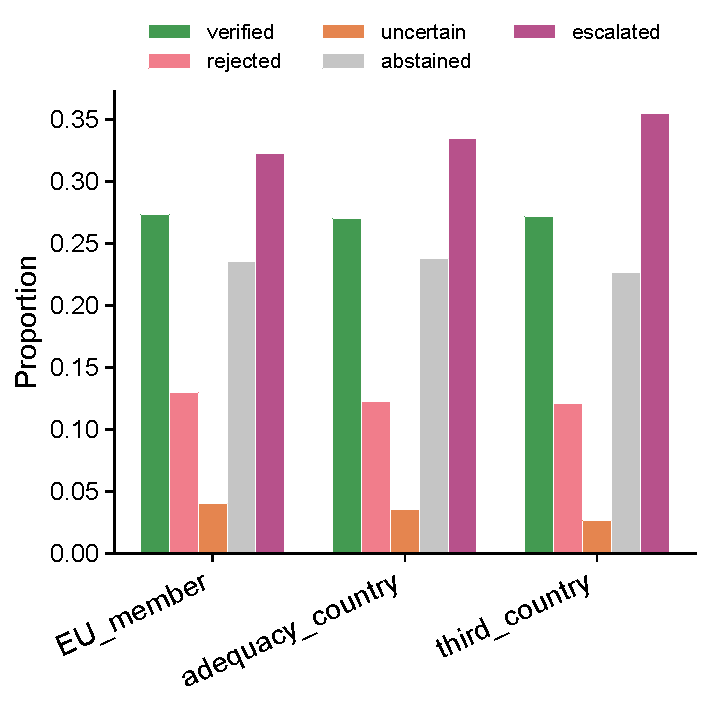
\includegraphics[width=\textwidth]{figure_show/Fig_10e.pdf}\end{subfigure}\hfill
\begin{subfigure}[t]{0.43\textwidth}\centering\footnotesize\textbf{Metadata quality ($m$)}\par\vspace{1pt}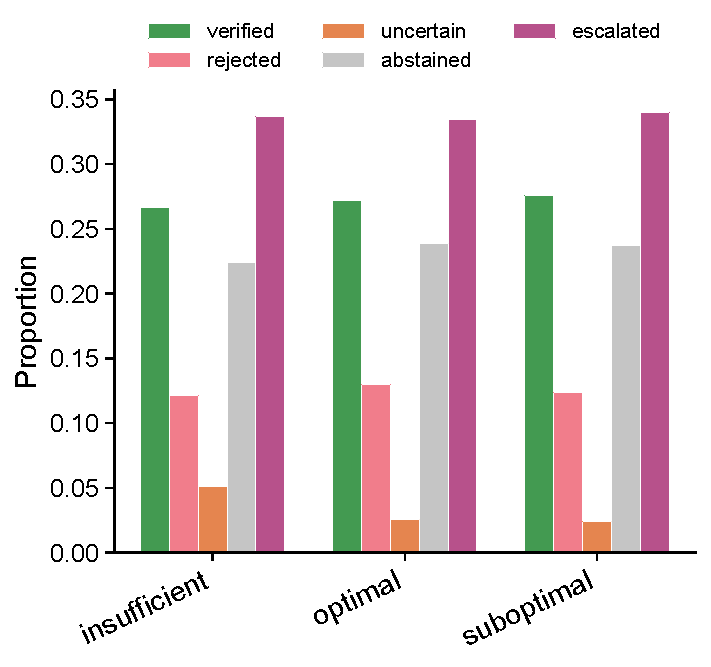
\includegraphics[width=\textwidth]{figure_show/Fig_10f.pdf}\end{subfigure}
\caption{Input feature impact on governance outcomes and stage progression. Bars show the proportion of terminal outputs stratified by each input feature.}
\label{fig:feature_impact}
\end{figure}

\subsection{Governance constraints operate as hard guarantees, not soft preferences}

A governance framework that merely recommends constraints without enforcing them provides no formal assurance: a policy could learn to violate governance rules in pursuit of higher reward. The pipeline MDP is designed so that critical governance constraints—stage-specific action availability, resource budgets, and compliance-driven penalties—are implemented as deterministic admissible-action filters and structural reward components rather than as learnable preferences (Table~\ref{tab:constraints}).

\begin{table}[t]
\centering
\caption{Governance constraints and reward penalties implemented in the pipeline MDP. Hard constraints are enforced through deterministic admissible-action filters; soft constraints are implemented through reward penalties.}
\small
\begin{tabular}{lll}
\hline
Constraint & Type & Specification \\
\hline
a\_verify availability & Hard & Only in M2, M3 \\
a\_defer availability & Hard & Only in M1, M2, M3 (not M4) \\
a\_escalate availability & Hard & $g_{\mathrm{conf}} < 0.70$, or $\text{eval\_count} \geq 3$ and $g_{\mathrm{conf}} < 0.85$ \\
a\_redact availability & Hard & $b \in \{\text{categorisation}, \text{remote\_id}\}$, redact\_count $< 1$ \\
a\_eval resource limit & Hard & Max 5 per stage \\
a\_mitig resource limit & Hard & Max 3 per stage \\
a\_verify resource limit & Hard & Max 3 per stage \\
a\_defer resource limit & Hard & Max 2 per stage \\
a\_redact resource limit & Hard & Max 1 per episode \\
\hline
Correct accept/reject & Reward & +50 each \\
Misclassification & Reward & $-$80 \\
False accept & Reward & $-$60 \\
False reject & Reward & $-$55 \\
Mitigation success (stage downgrade) & Reward & +12 \\
Escalation & Reward & $-$20 each \\
Correct abstain (high/prohibited) & Reward & $-$15 \\
Cross-border penalty (unmitigated) & Reward & $-$25 \\
Reckless decision (M3/M4, eval $< 2$) & Reward & $-$10 \\
Step cost & Reward & $-$1 per step \\
Consecutive defer penalty & Reward & $-$3 per extra defer \\
\hline
\end{tabular}
\label{tab:constraints}
\end{table}

The results confirmed that these constraints functioned as hard governance guarantees across all 33,331 episodes. No episode produced an invalid action. Verification was exclusively activated in M2 and M3, deferral was restricted to M1--M3, escalation required genuine uncertainty conditions ($g_{\mathrm{conf}} < 0.70$ or sustained low confidence despite multiple evaluations), and redaction was limited to categorisation and remote-identity basis types with a hard budget of one invocation. The zero violation rate across 441,808 state transitions establishes that the admissible-action filter constitutes a formal governance guarantee—the policy operates within a provably safe action subspace at every decision point.

Risk-adaptive governance mechanisms functioned as intended. Among the 5,622 high-risk and 13,897 prohibited-tier episodes, 62.0\% and 61.3\% respectively were routed to escalation or abstention rather than forced terminal decisions. The policy learned to suppress unsafe low-confidence decisions under elevated risk conditions, preferentially absorbing the moderate negative rewards associated with escalation ($-$20) and correct abstention ($-$15) rather than risking the severe penalties for false acceptance ($-$60) or misclassification ($-$80). In contrast, 46.8\% of minimal-risk and 47.2\% of limited-risk episodes reached terminal accept/reject decisions, with correct-decision rates of 69.4\% and 68.4\% respectively among those that did, demonstrating appropriately calibrated permissiveness for low-risk requests.

The cross-border compliance mechanism ($R_{\mathrm{XB\_PENALTY}} = -25$) provided an additional structural safeguard. This penalty was triggered when a decision involved non-compliant jurisdictions ($c \in \{\mathrm{non\_compliant}, \mathrm{inadequate\_SCC}\}$) without prior mitigation, creating a structured disincentive against ungoverned cross-border data flows. The penalty is not a learnable parameter but a deterministic function of state features, ensuring that cross-border compliance is architecturally enforced.

The escalation mechanism exhibited precisely the two-stage behaviour prescribed by its design. Although 35.8\% of episodes involved at least one escalation action, 99.2\% of these episodes culminated in terminal escalation upon the second invocation, consistent with the escalating-penalty structure that provides exactly one opportunity for uncertainty resolution before mandatory termination. This design prevents both infinite escalation loops—a critical failure mode in human-review referral systems—and premature termination that would deny the policy a reasonable opportunity to resolve ambiguity.

Together, these results demonstrate that the pipeline MDP governance framework supports: interpretable stage-dependent decision dynamics in which uncertainty is progressively characterised, bounded, and resolved through semantically distinct governance stages; probabilistically verifiable transition behaviour that enables trajectory-level audit and replay; and hard governance constraints that operate as formal guarantees rather than learnable preferences. The framework thus establishes a foundation for trustworthy AI governance in which semantic expressivity and operational uncertainty are not opposing forces to be traded off, but coupled dimensions of a formally constrained and empirically verifiable decision process.



\section{Discussion}

The results demonstrate that the proposed Markov decision framework provides a formally constrained mechanism for governing AI systems operating under uncertainty. Unlike conventional AI pipelines that optimise predictive performance without explicit governance semantics, the proposed approach maintains interpretable and probabilistically verifiable decision trajectories across sequential reasoning, verification, mitigation, and terminal decision states.

The observed transition dynamics reveal that the four sequential governance stages naturally develop distinct operational behaviours within the pipeline. Verification-oriented stages (M2) stabilised decision trajectories under low uncertainty, whereas multimodal fusion stages (M3) generated increased mitigation activity due to higher uncertainty propagation associated with heterogeneous biometric evidence. The most restrictive governance stage (M4) exhibited conservative transition policies and stronger convergence towards terminal validation and rejection under elevated regulatory-risk conditions. These stage-dependent dynamics indicate that the framework successfully balances semantic expressivity against bounded-risk operation through progressively restrictive governance.

The constrained policy formulation further ensured that unsafe or non-compliant actions were excluded from admissible execution pathways. Escalation, abstention, and mitigation actions were consistently activated under unresolved uncertainty or elevated regulatory-risk conditions, demonstrating operational enforcement of governance constraints rather than post hoc explainability alone.

From a regulatory perspective, the framework provides an explicit mechanism for implementing transparency, traceability, and risk-aware oversight requirements associated with high-risk AI systems under emerging governance frameworks including the European Union AI Act. More broadly, the proposed execution semantics establish a foundation for trustworthy and self-sovereign AI systems capable of operating across heterogeneous jurisdictions, modalities, and uncertainty conditions while preserving reproducibility, auditability, and constrained decision execution.


\section{Methods}

\subsection{System overview}

At decision epoch \(t\), the system receives a request \(x_t\) consisting of biometric inputs, contextual metadata, and previously accumulated evidence. Supported biometric modalities include facial, ear, fingerprint, iris, and voice recognition. A biometric subsystem transforms raw signals into modality-aware summaries including quality measures, similarity scores, calibrated confidence estimates, and uncertainty indicators. Additional evidence may include audit records, model documentation, consent status, provenance metadata, and cross-border transfer information.

All evidence is encoded into a structured control state \(s_t\). The policy controller selects an action \(a_t\), and an enforcement layer maps the selected action to the released outcome. Actions include acceptance, rejection, abstention, escalation, verification, mitigation, redaction, deferment, and compliance evaluation. The enforcement layer is deterministic and blocks actions violating hard admissibility constraints, applies pseudonymization or redaction where required, records state transitions for auditability, and ensures oversight obligations are satisfied.

\textit{\textbf{----FIGURE}}

\subsection{Formal MDP formulation}

The governance controller is defined as the Markov Decision Process
\begin{equation}
\mathcal{M}=(S,A,T,R,\gamma),
\end{equation}
where \(S\) denotes the state space, \(A\) the action space, \(T\) the transition kernel, \(R\) the expected one-step reward, and \(\gamma\in[0,1)\) the discount factor. Initial states are sampled from \(p_0(s)\), representing uncertainty over biometric modality, evidence completeness, jurisdictional context, and regulatory posture.

At epoch \(t\), the state is represented as
\begin{equation}
s_t=(d_t,b_t,q_t,m_t,\alpha_t,c_t,\rho_t,\zeta_t,u_t,j_t,k_t,g_t),
\end{equation}
where \(d_t\) denotes the data representation type, \(b_t\) the biometric modality, \(q_t\) the request category, \(m_t\) contextual metadata, \(\alpha_t\) calibrated confidence estimates, \(c_t\) compliance status, \(\rho_t\) privacy-risk indicators, \(\zeta_t\) Quality-of-Service indicators, \(u_t\) predictive uncertainty, \(j_t\) jurisdictional context, \(k_t\) workflow stage, and \(g_t\) the regulatory-tier belief vector.

The regulatory-tier belief vector is defined on the probability simplex
\begin{equation}
g_t\in\Delta^{|\mathcal{Y}|-1},
\qquad
\mathcal{Y}=
\{\mathrm{minimal},\mathrm{limited},\mathrm{high},\mathrm{prohibited}\},
\end{equation}
where \(g_t(y)\) denotes the belief that regulatory tier \(y\in\mathcal{Y}\) applies.

The action space is
\begin{equation}
A=
\{
a_{\mathrm{accept}},
a_{\mathrm{reject}},
a_{\mathrm{abstain}},
a_{\mathrm{defer}},
a_{\mathrm{verify}},
a_{\mathrm{redact}},
a_{\mathrm{escalate}},
a_{\mathrm{mitigate}},
a_{\mathrm{evaluate}}
\}.
\end{equation}

State evolution is governed by the transition kernel
\begin{equation}
T_{\theta}(s'\mid s,a)
=
\Pr(S_{t+1}=s'\mid S_t=s,A_t=a;\theta),
\end{equation}
where \(\theta\) denotes the transition parameterization. For discrete states,
\begin{equation}
\sum_{s'\in S}T_{\theta}(s'\mid s,a)=1.
\end{equation}
For continuous or hybrid state spaces,
\begin{equation}
\int_S T_{\theta}(ds'\mid s,a)=1.
\end{equation}

Transition dynamics capture stochastic evolution of uncertainty, evidence completeness, compliance status, and governance state. For example, \(a_{\mathrm{evaluate}}\) may reduce uncertainty and update \(g_t\), whereas \(a_{\mathrm{mitigate}}\) may reduce regulatory or privacy risk.

The true regulatory risk tier $y \in \mathcal{Y}$ is latent---computed from input features with additive noise but never directly observed by the agent. To handle this partial observability within a standard MDP formulation, the framework maintains a probabilistic belief vector $g_t \in \Delta^{|\mathcal{Y}|-1}$ over the regulatory tier, which is included in the state representation. The belief is initialised from observable input features via a score-based prior and updated through Bayesian evidence propagation when evaluation or verification actions are performed. Crucially, by encoding $g_t$ into the full state vector $s_t$, the problem reduces to a standard MDP over the augmented state space---the DQN learns $Q(s_t, a)$ where $s_t$ contains both observable features and the current belief. The Bayesian update thus serves as a state estimation mechanism rather than as part of POMDP planning (which would require solving a Belief MDP over the continuous belief simplex). This design preserves the formal interpretability of Bayesian inference while retaining the computational tractability of standard deep Q-learning.

When regulatory tier is latent, \(g_t\) is updated through Bayesian evidence propagation. Let \(e_{t+1}\) denote newly observed evidence and let
\begin{equation}
p_{\eta}(e_{t+1}\mid y,s_t,a_t)
\end{equation}
be the evidence likelihood under tier \(y\). The posterior belief update is
\begin{equation}
g_{t+1}(y)
=
\frac{
p_{\eta}(e_{t+1}\mid y,s_t,a_t)g_t(y)
}{
\sum_{y'\in\mathcal{Y}}
p_{\eta}(e_{t+1}\mid y',s_t,a_t)g_t(y')
}.
\end{equation}

The one-step reward is defined by
\begin{equation}
r_t\sim \rho(r\mid s_t,a_t,s_{t+1}),
\qquad
R(s,a,s')=\mathbb{E}_{\rho}[r\mid s,a,s'].
\end{equation}

The expected reward is
\begin{align}
R(s,a,s')
&=
w_u U(s,a,s')
-w_c C_{\mathrm{reg}}(s,a,s')
-w_p C_{\mathrm{priv}}(s,a,s') \nonumber\\
&\quad
-w_r C_{\mathrm{rob}}(s,a,s')
-w_f C_{\mathrm{fair}}(s,a,s')
-w_q C_{\mathrm{QoS}}(s,a,s'),
\end{align}
where \(U\) denotes task utility and the remaining terms represent regulatory, privacy, robustness, fairness, and Quality-of-Service costs.

Policy optimisation is formulated as a constrained MDP:
\begin{equation}
\pi^{\star}
\in
\arg\max_{\pi}
\mathbb{E}_{\pi}
\left[
\sum_{t=0}^{\infty}
\gamma^t R(S_t,A_t,S_{t+1})
\right],
\end{equation}
subject to
\begin{equation}
\mathbb{E}_{\pi}
\left[
\sum_{t=0}^{\infty}
\gamma^t C_i(S_t,A_t,S_{t+1})
\right]
\leq d_i,
\qquad i=1,\ldots,m.
\end{equation}

Hard constraints are represented through the admissible action set
\begin{equation}
A_{\mathrm{safe}}(s)
=
\{a\in A: h_j(s,a)\leq0,\ j=1,\ldots,k\},
\end{equation}
where \(h_j\) are regulatory, privacy, oversight, or safety predicates. Operational policies satisfy
\begin{equation}
\pi(a\mid s)=0
\qquad
\mathrm{for\ all}\quad
a\notin A_{\mathrm{safe}}(s).
\end{equation}

\subsection{Governance constraints and assurance mechanisms}

The framework distinguishes between hard and soft governance constraints. Hard constraints prohibit unsafe or non-compliant actions through admissible-action filtering and deterministic enforcement. These include prohibited biometric practices, missing oversight requirements, disallowed cross-border transfers, and unresolved compliance violations.

Soft constraints are represented through optimisation penalties and bounded cumulative costs, including fairness regularization, robustness penalties, latency, Quality-of-Service degradation, and privacy costs. Privacy budgets may additionally be constrained through
\begin{equation}
\epsilon_{\mathrm{cum}}\leq \epsilon_{\max}.
\end{equation}

The framework provides auditability through replayable state transitions, explicit uncertainty representation, evidence provenance tracking, and interpretable policy execution. Human oversight is incorporated through escalation and abstention actions when uncertainty or regulatory risk exceeds admissible thresholds.

\subsection{Simulation and reproducibility}

Transition probabilities were generated using documented rule-based transition matrices parameterised by governance stage, evidence completeness, uncertainty level, and regulatory risk tier. Simulated trajectories were sampled through stochastic policy execution over 33,331 independent decision episodes comprising 475,139 governance steps and 441,808 state transitions across four sequential governance stages (M1--M4) and ten action types.

Statistical analysis included transition probability estimation, Spearman correlation analysis, action-distribution profiling, transition heatmaps, force-directed state-transition graph visualisation, and feature impact analysis. All transition matrices, reward parameters, constraint definitions, and random seeds are reproducible from the released implementation and supplementary materials.

\subsection{Decision outputs}

Externally visible outputs are restricted to
\begin{equation}
O=
\{
\mathrm{verified},
\mathrm{rejected},
\mathrm{uncertain},
\mathrm{abstained},
\mathrm{escalated}
\}.
\end{equation}

The output \(\mathrm{verified}\) indicates that the selected policy satisfies the current governance constraints. The outputs \(\mathrm{uncertain}\), \(\mathrm{abstained}\), and \(\mathrm{escalated}\) preserve bounded-risk operation when evidence, uncertainty, or compliance conditions remain unresolved.

\section{Data availability}
All simulation data generated and analysed in this study are publicly available. The primary dataset, \texttt{results\_pipeline\_v1.csv} (33,331 episodes $\times$ 40 columns), records every governance trajectory with per-episode fields including the complete action path, final decision output, cumulative reward, belief-state vector, stage progression, action counts, and all input feature values. The aggregated transition dataset, \texttt{transition\_pipeline\_v1.csv}, provides the state--action--next-state transition counts used to construct all transition probability matrices, heatmaps, and force-directed graphs presented in Figs.~5--8. Both CSV files, together with a data dictionary documenting all column definitions and the random seeds used for stratified sampling, are available at \url{https://github.com/violector/CrossBorder} and are deposited in the Figshare repository. Source data underlying all figures can be regenerated from these files using the provided analysis scripts.

\section{Code availability}
The complete software implementation is open-source and available at \url{https://github.com/violector/CrossBorder} under the MIT License. The repository contains three main components: \texttt{cross\_pipeline\_mdp\_v1.py}, which implements the pipeline MDP environment, the 22-dimensional state encoder, the DQN agent with prioritised experience replay, the admissible-action filter, and the full reward structure (Table~\ref{tab:constraints}); \texttt{cross\_analysis\_pipeline\_split.py}, which reads the simulation outputs and generates all 40 individual panel figures as both PDF and PNG; and a \texttt{README.md} with step-by-step reproduction instructions, including Python dependency specifications (~\texttt{torch}, \texttt{numpy}, \texttt{pandas}, \texttt{matplotlib}, \texttt{seaborn}, \texttt{networkx}, \texttt{scipy}). All parameter values---transition probabilities, reward weights, resource budgets, constraint thresholds, and random seeds---are documented in the source code and can be inspected or modified. An interactive Google Colab notebook reproducing the core training and analysis pipeline without local installation is available at \url{https://colab.research.google.com/XXXXX}.

\section*{Acknowledgment}
The research and development reported in this paper have received funding from .... under grant agreement no. ..... (Project Name) and the Research Programme P2-0426, Digital Transformation for Smart Public Governance.

\bibliographystyle{...}

\begin{thebibliography}{widest entry}
 \bibitem[label1]{figshare} Hu, K. \textit{et al}. CrossBorder AI Governance --- Pipeline MDP Simulation Data. \textit{Figshare} \url{https://doi.org/XXXXX} (2026).
 \bibitem[label2]{cite_key2} bibliographic information
 ...
\end{thebibliography}

\end{document}





